\documentclass[upright, contnum]{umemoria}
\deptoA{DEPARTAMENTO DE INGENIERÍA ELÉCTRICA}
\deptoB{DEPARTAMENTO DE CIENCIAS DE LA COMPUTACIÓN}
\author{Matías Fernando Pavez Bahamondes}
\title{Diseño e Implementación de Memoria de Largo Plazo para Robots de Servicio}
\auspicio{}
\date{2018}
\guia{Javier Ruiz del Solar, JOCELYN SIMMONDS WAGEMANN}
\carreraA{INGENIERO CIVIL ELÉCTRICO E}
\carreraB{INGENIERO CIVIL EN COMPUTACIÓN}
\memoria{MEMORIA PARA OPTAR AL TÍTULO DE INGENIERO CIVIL ELÉCTRICO E INGENIERO CIVIL EN COMPUTACIÓN}
\comision{TODO 1, TODO 2, TODO 3}

\usepackage[T1]{fontenc}
\usepackage[spanish]{babelbib}
\usepackage{enumitem} % opciones para itemize 

% ------------- Imágenes -------------------------------------- %
\usepackage[pdftex]{graphicx}	% Para Archivos gráficos         %
\usepackage{float}				% Para usar H!                   %
\usepackage[section]{placeins}	% auto \FloatBarrier por sección %
\usepackage{caption}			% [font=small,labelfont=bf]      %
\usepackage{subcaption}         % Caption para subfiguras        %
\usepackage{sidecap}            % Captions al lado               %
\usepackage{wrapfig}            % Escribir alrededor             %
\graphicspath{{./figures/}}     % Agrega Path para buscar imgs.  %
% ------------------------------------------------------------- %

% = = = = = = = = = = = = = = = = = = = = = = =
% TODO NOTES
% = = = = = = = = = = = = = = = = = = = = = = =
\usepackage[pdftex,dvipsnames,table]{xcolor}  % Coloured text etc.
\usepackage{xargs} % Use more than one optional parameter in a new commands
\usepackage[colorinlistoftodos,prependcaption,textsize=small]{todonotes}
%\usepackage[colorinlistoftodos,prependcaption,textsize=tiny,disable]{todonotes}
\newcommandx{\unsure}[2][1=]{\todo[linecolor=red,backgroundcolor=red!25,bordercolor=red,#1]{#2}}
\newcommandx{\change}[2][1=]{\todo[linecolor=blue,backgroundcolor=blue!25,bordercolor=blue,#1]{#2}}
\newcommandx{\info}[2][1=]{\todo[linecolor=OliveGreen,backgroundcolor=OliveGreen!25,bordercolor=OliveGreen,#1]{#2}}
\newcommandx{\improvement}[2][1=]{\todo[linecolor=Plum,backgroundcolor=Plum!25,bordercolor=Plum,#1]{#2}}
\newcommandx{\thiswillnotshow}[2][1=]{\todo[disable,#1]{#2}}
\setlength{\marginparwidth}{0.5in}
% = = = = = = = = = = = = = = = = = = = = = = =


\hypersetup{
	colorlinks,
	linkcolor={black},
	citecolor={blue!50!black},
	urlcolor={blue!80!black}
}

%Para la Carta Gantt
\usepackage{gantt}
\usepackage{tikz}

\definecolor{Gray}{gray}{0.9}


\usepackage{lipsum}

\begin{document}

\frontmatter
\maketitle

\begin{abstract}
\todo[inline]{Abstract: Escribir al final.}
\end{abstract}

\begin{dedicatoria}
\todo[inline]{Escribir una dedicatoria corta}
\end{dedicatoria}

\begin{thanks}
\todo[inline]{Escribir agradecimientos}
\end{thanks}

\cleardoublepage
\tableofcontents
\cleardoublepage
\listoftables
\cleardoublepage
\listoffigures

\listoftodos

\mainmatter


\chapter{Introducci\'on}

\section{Antecedentes Generales}

A continuaci\'on se presenta una breve introducci\'on a los temas requeridos para contextualizar este trabajo de t\'itulo: La rob\'otica de servicio y el equipo de trabajo donde se implantar\'a la soluci\'on. Adem\'as, se introduce el tema de la memoria humana, requerido para entender la propuesta y su relaci\'on con la rob\'otica.


\subsection{Robots de servicio}

La rob\'otica de servicio es un \'area enfocada en asistir a los seres humanos en tareas repetitivas y comunes, como la recolecci\'on de basura. Formalmente, se define un \textit{robot de servicio} como un robot ``que realiza tareas \'utiles para humanos o equipamiento, excluyendo aplicaciones de automatizaci\'on industrial''\cite{IFR}. Luego, el robot requiere cierto grado de autonom\'ia, que es la habilidad de actuar a partir del estado actual, usando lo que observa del ambiente y sin intervenci\'on humana. As\'i, un robot de servicio debe trabajar en ambientes no controlados y con la autonom\'ia suficiente que le permita llevar a cabo su cometido.

Un caso de uso t\'ipico es la asistencia en las tareas del hogar, donde se espera que un robot pueda ayudar a ordenar, preparar comida u ofrecer bebestibles. Otros casos de uso consideran el cuidado de adultos mayores, robots para compa\~nia en el hogar, mascotas robots, salud o educaci\'on. Particularmente, la compa\~nia SoftBank Robotics es pionera en ofrecer a Pepper como el primer robot humanoide ya adoptado en hogares de Jap\'on, as\'i como robot de bienvenida en hoteles y tiendas\cite{softbank}.


\subsection{Equipo de Trabajo: UChile Homebreakers}

El laboratorio de rob\'otica del Departamento de Ingenier\'ia El\'ectrica de la Universidad de Chile alberga dos equipos de rob\'otica: \textit{UChile Robotics Team}, dedicado al f\'utbol rob\'otico y \textit{UChile Homebreakers Team}, enfocado en rob\'otica de servicio. Ambos son conformados por alumnos de pregrado y postgrado de diversas especialidades, y liderados por el profesor Javier Ruiz del Solar\cite{uchile-robotics}.

UChile Homebreakers existe desde el a\~no 2007 y actualmente cuenta con 15 estudiantes. Todo su desarrollo de software est\'a basado en ROS, un framework para el desarrollo de plataformas rob\'oticas y con miles de usuarios alrededor del mundo\cite{ROS:2009}.

El equipo trabaja en dos plataformas humanoides, Bender y Pepper. Bender es un robot construido en el mismo laboratorio y con el objetivo de ser un mayordomo para el hogar. Pepper, desarrollado por SoftBank Robotics, est\'a dise\~nado para ser un robot de compa\~nia. Ambos comparten la misma arquitectura de software y pr\'acticamente todo su c\'odigo, exceptuando los drivers para acceder al hardware respectivo.


\subsubsection{RoboCup @Home League}


La RoboCup es una competencia internacional cuyo objetivo es ser un veh\'iculo para el desarrollo de la rob\'otica y la inteligencia artificial. Est\'a compuesta de variadas ligas: Rescue, Soccer, Simulation, @Home, Industrial y Junior, cada una con diversas subligas orientadas a fomentar la investigaci\'on de distintos aspectos del campo. Su sue\~no es que para mediados del siglo 21, un equipo de f\'utbol rob\'otico completamente aut\'onomo sea capaz de vencer al campi\'on de la \'ultima copa mundial y siguiendo las reglas de la FIFA\cite{robocup:rulebook_2017}.

UChile Homebreakers participa desde el a\~no 2007 en la categor\'ia @Home. Las pruebas de la liga se desarrollan en escenarios que imitan ambientes reales, como un hogar o un restaurante. 
%Adem\'as, la competencia funciona como un espect\'aculo para p\'ublico general, por lo que se priorizan pruebas y demostraciones interesantes para los espectadores.
% 
Las capacidades generalmente evaluadas y potenciadas en @Home son de Vision Computacional, Navegaci\'on aut\'onoma, Manipulaci\'on de objetos y Reconocimiento de Voz. Cada a\~no el equipo planifica sus desarrollos de acuerdo a los requerimientos de la competencia, por lo que trabajos fuera de las \'areas mencionadas no son considerados una prioridad.


\subsection{La memoria humana}

La memoria hace relaci\'on al almacenamiento de experiencias en el cerebro. Hay m\'ultiples sistemas de memoria independientes y sustentados por distintas estructuras cerebrales. A grandes rasgos, la memoria se puede dividir en de corto plazo STM (Short-Term Memory) y de largo plazo LTM (Large-Term Memory). La STM maneja informaci\'on muy detallada, es de poca capacidad y permite un r\'apido acceso, mientras que la LTM maneja mucha informaci\'on sobre experiencias y entidades, es menos detallada y de acceso m\'as lento\cite{Eichenbaum:2008}.

La LTM se puede dividir en expl\'icita (consciente) e impl\'icita (inconsciente). La primera almacena datos epis\'odicos, pudiendo responder las preguntas ``Qu\'e'', ``D\'onde'' y ``Cu\'ando'', datos sem\'anticos, que modelan hechos y conceptos como el lenguaje o personas, y tambi\'en, las conexiones entre ambas submemorias. La memoria impl\'icita codifica habilidades, h\'abitos y preferencias.

Existen procesos de consolidaci\'on y deterioro de la memoria que est\'an constantemente en funcionamiento. La consolidaci\'on requiere un est\'imulo relevante, sumado al proceso de almacenamiento, lo que genera conexiones entre la memoria epis\'odica y la respectiva zona sem\'antica. En caso de haber experiencias repetidas, las conexiones se fortalecen. El deterioro de la memoria es un proceso que degenera las conexiones entre ambas formas de memorias expl\'icitas.

La memoria emocional es una forma de memoria impl\'icita que genera reacciones emocionales y sentimientos. Seg\'un los est\'imulos a los que se enfrente, permite modular el proceso de consolidaci\'on de la STM en LTM, modificando el nivel de relevancia de los eventos, pudiendo generar memorias muy fuertes y h\'abitos arraigados. Ejemplos de esto son los flashbacks y las memorias asociadas a eventos importantes.



\section{Motivaci\'on}

La memoria es una habilidad cognitiva crucial para los humanos. Al interactuar con otras personas o el ambiente les permite recordar experiencias pasadas y sus detalles. Luego, es de esperar que un robot de servicio posea una memoria que le permita potenciar sus capacidades de interaci\'on con los humanos que ayudar\'a\cite{Vijayakumar2014}. Una LTM permitir\'ia, por ejemplo, generar di\'alogos interesantes sobre eventos pasados o cosas que el robot puede inferir del comportamiento humano, por otro lado, tambi\'en permitir\'ia la generalizaci\'on de las tareas que tiene que llevar a cabo.

Particularmente, dado el enfoque de las plataformas a utilizar, Bender c\'omo robot mayordomo y Pepper c\'omo robot social, se espera que ambos posean capacidades avanzadas de interaci\'on con los humanos, para lo que se requiere una LTM.


\subsection{Problema}

El a\~no 2015 se desarroll\'o una LTM epis\'odica para el robot Bender, orientada a la interacci\'on con personas y objetos\cite{Sanchez:2015}. El trabajo consideraba m\'etodos para almacenar, adquirir y manejar la informaci\'on epos\'odica, sumado a un proceso simple de consolidaci\'on de memoria.

Actualmente la memoria desarrollada no est\'a operativa, ni es factible habilitarla. A continuaci\'on se listan los aspectos que se consideran causas del problema desde un punto de vista t\'ecnico y humano:
\begin{itemize}
\item No se integr\'o adecuadamente al software del robot, no se recopila ni provee informaci\'on continuamente mientras el robot est\'a en funcionamiento.
\item La memoria no provee una API que siga el est\'andar de los desarrollos del equipo, por lo que no se usa ni es mantenida.
\item RoboCup@Home no considera el uso de LTM en sus competencias, por lo que el equipo no tiene un incentivo real para seguir desarrollando o mantener la memoria. Esto adem\'as ha provocado que el c\'odigo quede obsoleto.
\end{itemize}

Por otro lado, suponiendo que lo anterior estuviese solucionado, a\'un existen los siguientes problemas:
\begin{itemize}
\item S\'olo considera 2 modelos sem\'anticos: Persona y Objeto, para los cuales s\'olo se almacena informaci\'on de nombre, nacionalidad e imagen.
\item A pesar de considerar un modelo para objetos, no se integr\'o con los m\'odulos relacionados que recopilan la informaci\'on, por lo que realmente la memoria s\'olo funciona para entidades de tipo Persona.
\item Es esperable que una memoria considere m\'as modelos (Personas, Objetos, Autos, Ni\~nos, Mascotas, etc) y m\'as caracter\'isticas para cada modelo (nombre, hobbies, trabajo, etc).
\item La consolidaci\'on de memoria STM a LTM s\'olo considera la primera interacci\'on con cada entidad, por lo que no existe actualizaci\'on de los datos.
\item Hay una restricci\'on en los modelos y caracter\'isticas a almacenar, respecto a la informaci\'on que el robot es realmente capaz de obtener.
\end{itemize}


\subsection{Oportunidad}

Existe un vasto desarrollo respecto a la memoria y los procesos cognitivos, sin embargo, la investigaci\'on se concentra en campos como psicolog\'ia, neurolog\'ia y ciencias cognitivas. 
Los estudios de LTM para robots de servicio son muy acotados y no existe una soluci\'on est\'andar a implementar. Algunos robots, como la versi\'on comercial de Pepper, utilizan LTM, pero el c\'odigo asociado no es libre, ni est\'a basado en ROS.

El uso de LTM no est\'a en las prioridades ``RoboCup'' del equipo, sino que es algo \'util para demostraciones y para potenciar la interacci\'on humano-robot. Por ello, se considera que no basta con desarrollar un m\'odulo capaz de recopilar informaci\'on inteligentemente, sino que adem\'as se requiere una integraci\'on con las capacidades de di\'alogo o de inferencia de informaci\'on, para finalmente proveer una demostraci\'on de \'estas habilidades.

As\'i, \'esta es una oportunidad para dise\~nar una LTM para robots de servicio, que considere aspectos como: 
\begin{itemize}
\item Memoria epis\'odica y sem\'antica adecuada a tareas generales de robots de servicio.
\item M\'etodolog\'ia para consolidaci\'on de STM en LTM.
\item Servicio para recopilaci\'on continua de informaci\'on
\item Implementaci\'on est\'andar ROS, adecuada a las plataformas donde se implantar\'a la soluci\'on.
%\item Capacidad de generar respaldos de la memoria y recuperaci\'on de \'estos. 
\item Memoria emocional que permita dar relevancia a los eventos.
\item Inferencia de informaci\'on a partir de datos de la memoria. Por ejemplo: ``Juan suele desayunar a las 9am'', ``El control de la TV suele estar en el sof\'a'', etc.
%\item Integraci\'on con el di\'alogo que realiza el robot.\unsure{quitarlo?}
\end{itemize}

Tanto la memoria emocional, como la inferencia de informaci\'on, se consideran requisitos deseables, por lo que est\'an fuera del \textit{core} del proyecto.

%Tambi\'en se considera que es la oportunidad de promover la inclusi\'on de desafios basados en LTM en la liga @Home, a partir de los resultados de \'este trabajo. As\'i, el desarrollo de LTMs y capacidades asociadas dejar\'ia de ser postergado y pasar\'ia a ser una prioridad para los equipos de la competencia.


%\subsection{Aporte del Trabajo}
%La contribuci\'on del trabajo es principalmente el dise\~no e implementaci\'on 
\todo[inline]{Contribuci\'on del trabajo}

\section{Objetivos}

\subsection{Objetivo General}

El objetivo general corresponde al dise\~no de una LTM para robots de servicio, que considere componentes epis\'odicos y sem\'anticos. La LTM debe ser integrada en Bender y Pepper, con un servicio en background que recopile informaci\'on y con una API acorde a los desarrollos de UChile Homebreakers. Adem\'as, la LTM debe quedar integrada con alguna demostraci\'on de \'esta capacidad, ya sea mediante el di\'alogo o mediante inferencia de informaci\'on.

En resumen, el producto final debe ser una LTM integrada en los robots, de generaci\'on continua de recuerdos y que provea una demostraci\'on de \'esta capacidad.


\subsection{Objetivos Espec\'ificos}

A continuaci\'on se presentan los objetivos espec\'ificos del trabajo, a modo de desglose del objetivo general en tareas m\'as acotadas.

\begin{itemize}
\item Definici\'on del proceso de consolidaci\'on de recuerdos.
\item Dise\~no de la arquitectura del sistema y validaci\'on
\item Implementaci\'on de la LTM y su API.
\item Servicio para recopilaci\'on continua de informaci\'on.
\item Implementaci\'on de la demostraci\'on.
\end{itemize}

Otros objetivos espec\'ificos, correspondientes a requisitos que no son del \textit{core} del proyecto, son la implementaci\'on de la memoria emocional y la implementaci\'on de un m\'odulo de inferencia de informaci\'on basada en LTM.


%\section{Alcances}
\todo[inline]{ALCANCES}

%\section{Estructura de la memoria}
\todo[inline]{ESTRUCTURA DE LA MEMORIA1}

\chapter{Marco Teórico}\label{chapter:theory}

En este capítulo se revisan los temas y conceptos teóricos relevantes para el desarrollo del trabajo. Se formaliza la definición de robot doméstico y sus alcances. Se describe la memoria humana, sus categorías, funcionamiento y procesos cerebrales relevantes. Basado en los temas anteriores, se revisa la relación entre robótica y la memoria humana: se describen algunos enfoques existentes y las reglas generales para su implementación.

%% =====================================================================
\section{Robots de Servicio Domésticos}\label{sec:domestic_robots}
%% =====================================================================
%% =====================================================================
%% =====================================================================
%% =====================================================================

La Federación Internacional de Robótica (IFR)~\cite{IFR} define \textit{robot} como:
\begin{quotation}
	``Un mecanismo actuado y programable en dos o más ejes y con un cierto grado de autonomía, que se mueve en su entorno para realizar tareas previstas. En este contexto, autonomía se refiere a la habilidad de realizar tareas previstas, basado en el estado actual y lo sensado, sin intervención humana.''
\end{quotation}

Asimismo, la IFR define un \textit{robot de servicio} como un robot ``que realiza tareas útiles para humanos o equipamiento, excluyendo aplicaciones de automatización industrial''. Así, un robot de servicio debe trabajar en ambientes no controlados y con la autonomía suficiente que le permita llevar a cabo su cometido. Generalmente, la robótica de servicio se enfoca en asistir a los seres humanos en tareas repetitivas y comunes.

Según su área de aplicación, un robot de servicio se clasifica en \textit{de uso personal} o \textit{de uso profesional}. Los primeros son utilizados en ambientes no comerciales y por personas comunes; como por ejemplo, un robot sirviente o una silla de ruedas autónoma. Un robot de servicio profesional se utiliza en ambientes comerciales, usualmente operados por alguien entrenado; un ejemplo son los robots de entrega de paquetes o para cirugía.

Según la recopilación de datos realizada por la IFR durante el 2016, este tipo de robots es utilizado en diversas áreas para tareas domésticas, entretenimiento, educación, investigación, asistencia a ancianos y discapacitados, transporte, seguridad y vigilancia. Finalmente, existen otros robots de servicio que no pueden ser clasificados en las categorías anteriores.

El foco de este trabajo son los robots de servicio personales, dedicados a tareas domésticas, clasificación a la que en  adelante se referirá como \textit{robots domésticos}.


%% =====================================================================

%% =====================================================================

%% =====================================================================

%% =====================================================================

%% =====================================================================

%% =====================================================================

%% =====================================================================

%% =====================================================================

%% =====================================================================
\section{Memoria Humana}\label{sec:human_memory}
%% =====================================================================
%% =====================================================================
%% =====================================================================
%% =====================================================================

La memoria es un elemento fundamental para los humanos en su día a día, es parte integral de su existencia. Permite recordar quién, qué, cómo, dónde y cuándo. En términos psicológicos, es la habilidad para codificar, almacenar y luego obtener información sobre eventos pasados, en el cerebro. Los pensamientos son parte de la memoria de corto plazo, mientras que eventos pasados son almacenados en una memoria de largo plazo. Existen muchos estudios en el área de la psicología cognitiva con diversas descripciones y modelos teóricos de cada tipo de memoria~\cite{Vijayakumar2014}.

Desde el punto de vista de la información procesada, la memoria es vista como una facultad humana consistente en procesos para el manejo de información. Los 3 componentes principales son:

\begin{itemize}[topsep=0pt]
	\setlength\itemsep{0.2em}
	\item \textbf{Codificación}: En este paso, se adquiere nueva información desde los sentidos humanos. Los datos son convertidos a un formato que pueda ser almacenado en la estructura cerebral correspondiente.
	\item \textbf{Almacenamiento}: Consiste en la creación de registros permanentes de información. Es un proceso pasivo, de continuo procesamiento para clasificar datos nuevos y los ya existentes en el cerebro.
	\item \textbf{Adquisición}: Hace referencia al acceso de datos almacenados. El proceso se realiza en respuesta a una pista, que permita obtener una reconstrucción aproximada de la información, a partir de elementos repartidos en distintas partes del cerebro.
\end{itemize}
%\bigskip

La memoria puede ser dividida en múltiples sistemas independientes, con funcionalidades bien definidas y sustentados por distintas estructuras cerebrales~\cite{pmid-Squire}. La primera diferenciación define dos tipos de memoria: la de corto y la de largo plazo, STM (Short-Term Memory) y LTM (Long-Term Memory), por sus siglas en inglés~\cite{pmid10643472}. En el diagrama de la Figura~\ref{img:human_memory} se muestra una separación clásica utilizada en el área de las ciencias cognitivas~\cite{Eichenbaum:2008}, explicada en las siguientes subsecciones.

\usetikzlibrary{arrows,shapes,positioning,shadows,trees}
\tikzset{
	basic/.style  = {draw, drop shadow, font=\sffamily, rectangle},
	root/.style   = {basic, rounded corners=2pt, text width=10em, very thick, align=center, fill=gray!10},
	level 1/.style = {sibling distance=20mm},
	level 2/.style = {basic, rounded corners=6pt, thick,align=center, fill=gray!20, text width=8em},
	level 3/.style = {basic, rounded corners=2pt, thick, align=center, fill=gray!10, text width=6.5em},
	level 4/.style = {basic, thin, align=left, fill=gray!5, text width=10em}
}

\begin{figure}[!ht]
	\centering
	\begin{tikzpicture}[]
	
	\node [root] {Memoria Humana}
	child { node [level 2, xshift=-70pt] (c1) {\footnotesize Corto Plazo\\ (STM) }}
	child { node [level 2, xshift=100pt] (c2) {\footnotesize Largo Plazo\\ (LTM) }};
	
	\begin{scope}[every node/.style={level 3}]
	\node [below of = c2, xshift=-80pt, yshift=-20pt] (c21) {\footnotesize Explícita\\ (consciente)};  
	\node [below of = c2, xshift=80pt, yshift=-20pt] (c22) {\footnotesize Implícita\\ (inconsciente)};
	\end{scope} 
	
	\begin{scope}[every node/.style={level 4}]
	\node [below of = c21, xshift=40pt, yshift=-10pt] (c211) {\footnotesize Episódica};
	\node [below of = c211, xshift=0pt, yshift=0pt] (c212) {\footnotesize Semántica};
	
	\node [below of = c22, xshift=40pt, yshift=-10pt] (c221) {\footnotesize Procedural};
	\node [below of = c221, xshift=0pt, yshift=0pt] (c222) {\footnotesize Primado};
	\node [below of = c222, xshift=0pt, yshift=0pt] (c223) {\footnotesize Emocional};
	\end{scope} 
	
	\draw[-, to path={-- (\tikztotarget)}]
	(c2) edge (c21)
	(c2) edge (c22);
	
	\draw[-, to path={|- (\tikztotarget)}]
	(c21.195) edge (c211.west)
	(c21.195) edge (c212.west);
	
	\draw[-, to path={|- (\tikztotarget)}]
	(c22.195) edge (c221.west)
	(c22.195) edge (c222.west)
	(c22.195) edge (c223.west);
	
	\end{tikzpicture}
	\caption[Clasificaciones de la memoria humana.]
	{\small Clasificaciones de la memoria humana. Adaptado de~\cite{Vijayakumar2014}.}
	\label{img:human_memory}
\end{figure}



%% =====================================================================
%% =====================================================================
%% =====================================================================
\subsection{Memoria de corto plazo (STM)}
%% =====================================================================
%% =====================================================================
%% =====================================================================


En el ámbito cognitivo, la STM se refiere a la habilidad de estar atento, recopilar información  y memorias, para luego utilizarlas dentro de un corto periodo de tiempo~\cite{Eichenbaum:2008}. Es responsable de almacenar información constantemente y de decidir que parte será transferida a la LTM. El término de \textit{Memoria de Trabajo} suele ser utilizado de manera intercambiable con el de STM.

Se caracteriza por manejar información muy detallada, ser de poca capacidad y permitir un rápido acceso a estos datos. Permite recordar rápidamente y con gran detalle experiencias ocurridas hace pocos segundos, pero con dificultad creciente a medida que avanza el tiempo.

Se sustenta principalmente en la corteza prefrontal del cerebro. Las neuronas involucradas son capaces de mantener información relevante de corto plazo, la que es combinada con información sensorial entrante y áreas que manejan la toma de decisiones~\cite{Eichenbaum:2008}. 

En los humanos esta área presenta gran activación durante procesos de codificación, acceso y manipulación de memorias.


%% =====================================================================
%% =====================================================================
%% =====================================================================
\subsection{Memoria de largo plazo (LTM)}
%% =====================================================================
%% =====================================================================
%% =====================================================================


La LTM se asocia al almacenamiento permanente de información en el cerebro. Se caracteriza por manejar una gran cantidad de experiencias y entidades, ser menos detallada y proveer un acceso más lento a los recuerdos, respecto a la STM~\cite{Eichenbaum:2008}. Cierta información de la STM eventualmente es transferida a la LTM. De acuerdo a la Figura~\ref{img:human_memory}, sus dos principales categorías son la \textit{Memoria Implícita} y la \textit{Memoria Explícita}.


\subsubsection{LTM explícita}
%% =====================================================================

La memoria explícita suele ser denominada \textit{memoria consciente} o \textit{memoria declarativa}, pues maneja conocimientos relacionados a hechos y eventos adquiridos de forma consciente. Según las estructuras cerebrales involucradas, se conforma de la \textit{memoria episódica} y de la \textit{memoria semántica}~\cite{Eichenbaum:2008}.

La memoria episódica, por primera vez definida por Tulving~\cite{2_tulving}, es de carácter  autobiográfico y almacena detalles de eventos y experiencias pasadas. Permite responder a las preguntas ``Qué sucedió'', ``Dónde ocurrió'' y ``Cuándo ocurrió''~\cite{Deutsch2008}. Particularmente, se utiliza la noción de memoria episódica descrita por Clayton y Russel~\cite{CLAYTON20092330}, que incorpora el concepto de perspectiva episódica de los recuerdos. Un humano puede acceder a esta memoria si es capaz de decir: ``recuerdo que''. Este tipo de memoria da al ser humano la sensación de continuidad en el tiempo.

La memoria semántica almacena el conocimiento de hechos, significados, categorías y proposiciones. Un humano puede acceder a esta memoria si es capaz de decir: ``sé que''. Esta memoria se abstrae de perspectiva e información situacional.

Las estructuras cerebrales que soportan la memoria explícita son el hipocampo, encargado de manejar la memoria episódica, junto a la corteza cerebral, en donde se distribuyen los conocimientos de la memoria semántica. En el hipocampo se mantienen conexiones neuronales a los sectores de interés de la corteza, en donde se alojan conocimientos semánticos asociados a cada episodio.

Un ejemplo de uso de memoria episódica es el recuerdo de una graduación escolar, el lugar y la fecha donde ocurrió. La memoria semántica podría responder en que consiste una graduación y describir la ropa que se suele ocupar en ellas.



\subsubsection{LTM implícita}
%% =====================================================================

La memoria implícita abarca la capacidad de aprender habilidades, hábitos y preferencias, caracterizados por ser mejorados o adquiridos sin una recolección consciente. Así, también suele ser denominada \textit{memoria inconsciente} o \textit{memoria no declarativa}, pues comprende acciones que pueden ser realizadas sin pensar en ellas. Ejemplos de esto, son el andar en bicicleta o tocar un instrumento musical~\cite{Eichenbaum:2008}.

Dos de sus componentes son la \textit{memoria procedural} y la \textit{memoria de primado}. La primera ayuda a realizar tareas sin pensar en ellas, es decir, maneja el conocimiento del \textit{Cómo}; Ejemplos de esto son comer y caminar. La memoria de primado hace referencia a la predisposición para recordar hechos o información a la que un sujeto es expuesto con anterioridad; Ejemplos de esto son la facilidad para recordar canciones escuchadas hace poco tiempo, o el uso de palabras e ideas vistas recientemente.

Se ha mostrado que la memoria procedural se sustenta en el cerebelo, mediante la activación de este durante el uso de habilidades motoras.

Un tercer componente de la memoria implícita es la \textit{memoria emocional}. Esta se encarga de dar significado afectivo a ciertos estímulos, que de otra forma serían neutrales. Las estructuras cerebrales involucradas son la amígdala, las áreas corticales y subcorticales. Esta memoria se expresa mediante la activación del hipotálamo, en conjunto al sistema nervioso simpático, generando reacciones emocionales y sentimientos~\cite{episodic_philip}.


\subsection{Plasticidad sináptica y modulación}
%% =====================================================================

Se denomina \textit{consolidación} de memoria al proceso de transición de conocimiento desde la STM a la LTM~\cite{Bailey13445}. Durante la consolidación se generan conexiones neuronales entre la memoria episódica y la respectiva zona semántica. Para activar la consolidación se requiere de un estímulo relevante, sumado a la cadena de eventos para el almacenamiento~\cite{Eichenbaum:2008}.

Se denomina \textit{deterioro} de memoria u ``olvido'' al proceso de debilitamiento de las conexiones neuronales establecidas por los procesos de consolidación. Está en constante funcionamiento, degenerando las asociaciones entre la memoria episódica y la semántica. Por lo tanto, en este contexto, el olvido no significa una eliminación de los datos en el cerebro, sino que estos siguen ahí, pero la conexión requerida es inexistente o es demasiado débil para poder utilizarla.

Existen procesos químicos a nivel cerebral que afectan la consolidación y el deterioro de la LTM. Hay evidencia de que estos están en continuo funcionamiento. Estos eventos celulares ocurren en una escala de segundos a minutos, y son esenciales para la mantención de la LTM.

Es posible modular ambos procesos. Las experiencias repetidas potencian la consolidación de la memoria, lo que fortalece las conexiones neuronales. Por otro lado, la memoria emocional es capaz de potenciar o deprimir las reacciones químicas requeridas; según los estímulos a los que se enfrente, modifica el nivel de relevancia de los eventos, pudiendo generar memorias muy fuertes y hábitos arraigados. Ejemplos de esto, son la memorización por repetición, los flashbacks y las memorias asociadas a eventos importantes como cumpleaños.

%% =====================================================================

%% =====================================================================

%% =====================================================================

%% =====================================================================

%% =====================================================================

%% =====================================================================

%% =====================================================================

%% =====================================================================

\section{Memoria y Robótica}\label{sec:robotic_memory}
%% =====================================================================
%% =====================================================================
%% =====================================================================
%% =====================================================================
%% =====================================================================

En esta sección se revisan trabajos que buscan implementar LTM en robots. Se inicia haciendo énfasis en la importancia de esta en el campo de la robótica doméstica. Se hace una comparación entre la memoria humana y el manejo de información en robots. Luego, se revisan sistemas LTM encontrados en la literatura. Finalmente, se detallan las bases teóricas utilizadas para el diseño del proyecto, seleccionadas a partir de los trabajos más relevantes estudiados.


%% =====================================================================
%% =====================================================================
%% =====================================================================
\subsection{Relevancia de la LTM en robótica}
%% =====================================================================
%% =====================================================================
%% =====================================================================

% Ser Social e Interacciones
La LTM es una habilidad cognitiva esencial para cualquier ser social, otorgando una sensación de continuidad a la vida~\cite{Vijayakumar2014}. Durante una interacción social, permite recordar experiencias pasadas y relacionarlas con información actual, lo que genera interacciones interesantes y no monótonas. Lo mismo se aplica al caso de un robot doméstico, donde es esperable que posea una memoria que le permita establecer una relación de largo plazo con humanos, y potenciar sus capacidades de interacción con ellos.

% Robot SIN LTM
Para los desarrolladores, un problema común es que los usuarios tienden a perder el interés rápidamente en sus robots, pues existen expectativas no cumplidas respecto a la inteligencia y capacidad de socializar de la máquina~\cite{Ho2009}. El problema se potencia con el paso del tiempo, donde la motivación por interactuar disminuye y se genera frustración, a medida que el robot continua repitiendo los mismos comportamientos predefinidos. De manera similar para un humano, cuando la LTM no funciona correctamente debido a una enfermedad (por ejemplo, Alzheimer), la habilidad de interacción con otros humanos se ve dañada severamente~\cite{ltm_in_robocup}.

% Ventajas de LTM
Si se desea mejorar la interacción humano-robot, entonces se requiere que el robot se comporte de manera más natural. Los mejores agentes robóticos sociales deberían satisfacer las necesidades cognitivas y sociales humanas; mientras más familiar sea la interacción, serán más efectivos en su propósito. Así, la LTM es una habilidad crucial si se espera que el robot sea capaz de aprender y adaptarse a su entorno. Una LTM permitiría, por ejemplo, generar diálogos interesantes sobre eventos pasados o inferir aspectos del comportamiento humano, por otro lado, también permitiría la generalización de las tareas que tiene que llevar a cabo.

% Intentos
Durante la última década han habido algunos intentos de implementar LTM en robots domésticos, sin embargo, no existe una solución estándar y aún quedan muchas consultas sin responder~\cite{ltm_in_robocup}. Por ejemplo, no existe una estrategia clara para el almacenamiento de eventos y experiencias en la forma de episodios en una memoria LTM. Tampoco está claro como almacenar el estado emocional del robot y utilizarlo para modulación de la relevancia episódica. Otros puntos en investigación son la forma de consolidar la STM en LTM, la implementación de mecanismos de olvido y represión, y como manejar los aspectos éticos de adquirir y almacenar información personal de usuarios.

% Historias de Éxito
Por otro lado, desde un punto de vista práctico, se ha mostrado que el concepto de memoria LTM aplicada a robots es beneficioso. Salgado et al.~\cite{Salgado2012} ocupan memoria procedural para mejorar el desempeño de un robot en ambientes dinámicos, logrando acelerar el proceso de adaptación al entorno y la toma de decisiones.


%%% =====================================================================
%%% =====================================================================
%%% =====================================================================
%\subsection{Relación entre la memoria humana y la memoria robótica}
%%% =====================================================================
%%% =====================================================================
%%% =====================================================================
%
%Son muchos los trabajos en LTM que han basado su desarrollo en la taxonomía de la memoria humana, donde se implementan esquemas de información con módulos análogos a los presentados en la Figura~\ref{img:human_memory}. Esto se puede justificar por la similitud de cada tipo de memoria, con módulos preexistentes en la arquitectura robótica. A continuación se presenta una comparación entre cada tipo de memoria, sus procesos y el análogo robótico.
%
%\subsubsection{Memoria STM}
%Se relaciona a todos los datos que están actualmente cargados en la memoria primaria de la máquina. Esta memoria es la utilizada para solucionar la tarea actual, es equivalente a los pensamientos del robot y cumple con las características de la STM humana: es volátil, de rápido acceso y limitada en capacidad. También se encuentra presente en todo archivo temporal manejado por el sistema, mientras está en funcionamiento. Así, la estructura equivalente a la cerebral sería principalmente la RAM de la máquina y los archivos temporales.
%
%\subsubsection{Memoria Semántica}
%La memoria semántica es común y se puede asociar a casi toda fuente de datos estática, no utilizada por las otras memorias. Luego, la memoria semántica se sustenta en la memoria secundaria, cumpliendo las características de su análogo en los humanos: es persistente, de acceso costoso y virtualmente ilimitada en capacidad. En general, todo archivo con datos persistentes, utilizados para el funcionamiento del robot se podría considerar en esta categoría. Algunos ejemplos son:
%\begin{itemize}
%	\item Bases de datos.
%	\item Directorios con imágenes de personas y objetos conocidos.
%	\item Mapas con descripción del ambiente.
%	\item Archivos de audio utilizados por el robot.
%\end{itemize}
%
%
%\subsubsection{Memoria Procedural}
%Este tipo de memoria es comparable a algoritmos predefinidos para realizar acciones, generalmente motoras. Las estructuras equivalentes a la versión cerebral serían los archivos con parámetros para cada algoritmo, obtenidos a partir del entrenamiento o ajustados manualmente. Algunos ejemplos comparables son: 
%\begin{itemize}
%	\item Algoritmos basados en redes neuronales, entrenados para manipular objetos o reconocer patrones.
%	\item Algoritmos entrenados para tareas específicas, cómo la detección de caras o el reconocimiento de voz.
%	\item Controladores basados en puntos de operación para acciones motoras.
%	\item Síntesis de voz.
%\end{itemize}
%
%
%\subsubsection{Otros tipos de memoria}
%Generalmente, las memorias STM, semántica y procedural son un requisito mínimo para el funcionamiento de un software robótico, pero no son implementadas de forma explícita, sino que se pueden identificar en los componentes de software descritos anteriormente. Luego, la existencia de tales memorias, no implica la intención de crear una arquitectura LTM similar a la humana. Los otros tipos de memorias solo son implementados en casos especializados.
%
%

%% =====================================================================
%% =====================================================================
%% =====================================================================
\subsection{Revisión de sistemas LTM}\label{sec:revision_LTM}
%% =====================================================================
%% =====================================================================
%% =====================================================================
% - frameworks
% - trabajos relacionados
% - otros aspectos

A continuación se presenta una revisión de sistemas LTM basados en la memoria humana. En primer lugar se describen otras implementaciones de estos sistemas. Luego, se estudian trabajos con aspectos de interés para un sistema LTM. Para concluir, se muestran algunos trabajos enfocados en aspectos interesantes, pero que escapan de los alcances del proyecto.

\subsubsection{Frameworks LTM}

\ltmconcept{SOAR-EM (2004)} 
% Más info en: Sanchez:2015 , Stachowicz2012 , Deutsch2008
% About
Nuxoll y Laird presentaron SOAR-EM~\cite{Nuxoll2004ACM}, una extensión con memoria episódica para la arquitectura SOAR~\cite{LAIRD19871}. Ellos desarrollaron un sistema similar a PACMAN, donde la máquina debe moverse a través de una grilla para buscar ``comida'' lo más rápido posible. Utilizaron la memoria episódica para dar apoyo en la planificación de los movimientos del agente, mostrando que aquellos equipados con memoria episódica tienen un mejor desempeño que los que carecen de ella. 

% Episodios y limitantes
En SOAR-EM un episodio es creado con datos de la STM por cada acción del agente, los que pueden ser recolectados a partir de una pista episódica. Sin embargo, más adelante se mostró que el mecanismo de recolección es ineficiente y difícil de optimizar~\cite{Nuxoll2007}. Por otro lado, el trabajo no considera aspectos como el olvido episódico, ni la interacción de emociones con la LTM.


\ltmconcept{ISAC (2005)}
% Más info en: Sanchez:2015 , Stachowicz2012 , Deutsch2008
En el año 2005 Ratanaswasd et al.~\cite{Ratanaswasd2005} agregan memoria episódica al robot humanoide ISAC (Intelligent Soft Arm Control), enfocado en la manipulación de objetos. Los episodios son almacenados por su fecha y hora, combinados con todos los contenidos semánticos que aparecen en ese lapso. Luego, estos son recolectados para soportar la toma de decisiones en la planificación de trayectorias robóticas, bajo la suposición de que siempre existirá un episodio lo suficientemente similar a la situación actual. Más tarde, Dodd y Gutierrez~\cite{Dodd2005} incorporaron el concepto de relevancia emocional e histórica, con el objetivo de optimizar la búsqueda y eliminación de eventos según su intensidad. La relevancia emocional se obtiene directamente desde el sistema emocional de ISAC. Para la relevancia histórica, los eventos recientes son más importantes que los pasados, y experiencias novedosas tienen mayor puntaje que las comunes.

Los datos almacenados cubren el Qué, Cuándo y Dónde requeridos por Clayton~\cite{CLAYTON20092330}. Sin embargo, el diseño no provee la flexibilidad esperada en un sistema de memoria episódica:  Delimita los episodios por cambios en los objetivos generales de planificación del robot. No soporta el traslape ni la anidación de eventos. No queda claro si es suficientemente eficiente o escalable para cumplir con los requerimientos de un sistema episódico~\cite{Stachowicz2012}.

\ltmconcept{EPIROME (2008)} 
% Más información en:~\cite{Sanchez:2015}, Stachowicz2012
TASER es un robot de servicio enfocado a ambientes reales de oficina~\cite{Jockel2007}. Jockel et al.~\cite{Jockel2008} proponen el uso de memoria episódica para apoyar con tareas y evitar trabajo innecesario. Por ejemplo, al revisar oficinas para ayudar buscando personas, podría evitar las que usualmente están vacías. Para ello, Jockel et al. desarrollaron el framework EPIROME. Sus simulaciones mostraron que los agentes con memoria episódica se adaptan más rápido a nuevas situaciones que aquellos que carecen de ella.

A partir sus características, EPIROME no cumple con los requerimientos de un sistema de memoria episódica: No dispone de almacenamiento de largo plazo, mecanismos de recolección de episodios, ni representaciones de los eventos almacenados~\cite{Stachowicz2012}.

\ltmconcept{ALIZ-E (2014)}
ALIZ-E (Adaptative Strategies for Sustainable Long-Term Social Interaction) es un sistema cognitivo enfocado en la interacción natural con niños. Vijayakumar desarrolló una extensión de memoria episódica para ALIZ-E, basado en el funcionamiento de la memoria humana~\cite{Vijayakumar2014}. Su módulo construye episodios en formato RDF (Resource Description Framework), a partir de los archivos de \textit{log} que genera el sistema tras cada interacción.

Vijayakumar muestra que su sistema cumple con los requisitos de eficiencia esperados para su plataforma objetivo. Sin embargo, no aborda el diseño de metodologías para adquisición de episodios, ni la definición de información semántica, pues se enfoca en adaptar los archivos de \textit{log} preexistentes. Por otro lado, propone un caso de uso interesante para un robot social, a través de la adaptación de sus frases, según la información episódica almacenada, e.g., cambiando la frase ``Estoy feliz de verte'' a ``Estoy feliz de verte \textit{nuevamente}''. 


\ltmconcept{Bender}
El año 2015 Sanchez et al.~\cite{Sanchez:2015} diseñaron un sistema de memoria episódica para el robot Bender (plataforma de este proyecto). Este primer acercamiento es descrito en detalle en la Sección~\ref{sec:primer_acercamiento} y es utilizado como parte de la motivación para este proyecto.


\ltmconcept{Otros trabajos}
Existen otros esfuerzos en equipar robots con memoria episódica, por ejemplo, MINERVA2~\cite{Douglas1988}, LIDA~\cite{Feinstone2006}, Rity~\cite{Kuppuswamy2006}, Homer~\cite{Vere1990} y personajes de historias virtuales~\cite{Brom2007}. De manera similar a los trabajos descritos anteriormente, la mayoría de estos sistemas ha sido diseñado para satisfacer un contexto particular, por lo que no son útiles para el diseño de nuevos sistemas cognitivos robóticos~\cite{Stachowicz2012}.

% -~\cite{Pratama2014} ??
% - MINERVA 2 (1988)~\cite{Douglas1988}.  Más información en~\cite{Jockel2008}.
% - LIDA (2006)~\cite{Feinstone2006} % Más información:~\cite{Jockel2008}
% - Tecuci (2005)  % Más información: Deutsch2008
% D. Tecuci, “A generic episodic memory module,” University of Texas at Austin, Tech. Rep., 2005.D. Tecuci, “A generic episodic memory module,” University of Texas at Austin, Tech. Rep., 2005.



%\todoimprove{Agregar tabla indicando pros/cons de cada sistema LTM}


%\subsubsection{Procesos de consolidación y deterioro}
%
%%%- algunos solo procuran desarrollar reglas sobre como actualizar los pesos de aprendizaje
%% - dejar de aprender (sorprenderse al ser mayor)
%% - si no se implementa olvido, entonces la busqueda de informacion seria cada vez mas compleja.~\cite{Deutsch2008}
%
%
%%\todounsure{Hablar sobre este paper: sueño y postprocesamiento, puede estar demás para el marco teórico...}
%
%En un esquema LTM, un episodio puede estar constituido de muchos eventos, pero no todos son igualmente relevantes. En su trabajo, Kelley~\cite{Kelley2014} estudia 3 estrategias para la consolidación de recuerdos. La primera almacena todos los eventos ocurridos, pero tiene un costo de búsqueda lineal, respecto a los eventos almacenados; esta estrategia es impráctica a largo plazo. La segunda solo almacena eventos interesantes y realiza una búsqueda entre los más recientes; esta estrategia es práctica, pero no permite abstracción del evento. La tercera estrategia se basa en un postprocesamiento de las memorias, de manera similar al sueño humano.
%
%La estrategia propuesta por Kelley se basa en recordar todos los eventos, pero realizando un postprocesamiento de los datos una vez terminado el episodio. La ventaja es que no solo permite recordar los eventos interesantes del episodio, sino que además permite reconocer pistas o estímulos previos que sirven para prevenir un evento indeseado o potenciar eventos interesantes. Además, permite almacenar eventos posteriores, que sirven para entender las consecuencias del evento de interés. 
%
%En la Figura~\ref{img:sleep_eventos} se muestra un episodio conformado de una secuencia de 9 eventos. Entre los marcadores 1-2 y 5-6 hay eventos considerados poco interesantes, mientras que los eventos entre 3-4 son interesantes. Kelley propone almacenar la secuencia completa de eventos, para descartar los que no son útiles en un postprocesamiento. A priori se deben quitar los eventos entre 1-2 y 5-6, sin embargo, el evento 2 se mantiene en la memoria episódica como pista, y el evento 5 se mantiene para reforzar la consecuencia del episodio. Los resultados se pueden utilizar para aprendizaje reforzado, mientras que las pistas sirven para generalizar el episodio, en caso de que sean recurrentes.
%
%\begin{figure}[!ht]
%	\centering
%	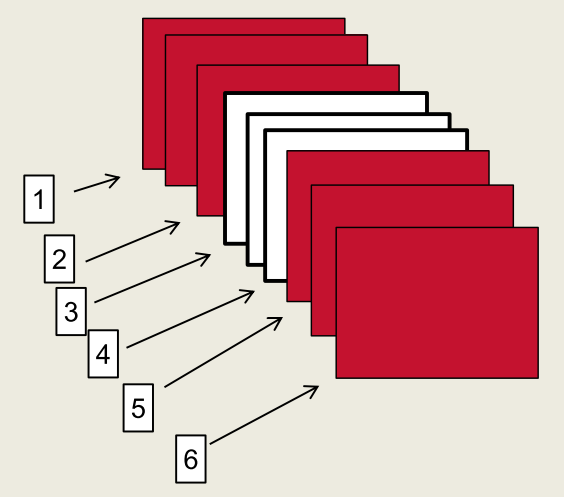
\includegraphics[width=0.4\textwidth]{eventos.png}
%	\caption{\small Ejemplo de una secuencia de eventos. Los cuadros coloreados y blancos indican eventos con poca o mucha relevancia, respectivamente. Los marcadores indican transiciones entre fases de poco y mucho interés. Obtenido de~\cite{Kelley2014}.}
%	\label{img:sleep_eventos}
%\end{figure}
%
%%Ejemplo:
%%At some location (cue), something big and orange (Tiger) moved from left to right resulting in pain (event)
%
%Además, este diseño permite que el sistema cambie su opinión sobre un evento, mediante aprendizaje reforzado. Si se repiten eventos, pero la consecuencia deja de ser la misma, entonces el sistema se acostumbra.


\subsubsection{Aspectos fuera del alcance del proyecto}\label{sec:otros_aspectos}
%% =====================================================================

A continuación se presentan algunos estudios relacionados con aspectos de una LTM que escapan de los requerimientos para este proyecto o que simplemente no son basados en la taxonomía de la memoria humana. Estos trabajos solo se presentan a modo de completitud, pues no permiten resolver el objetivo de este proyecto, sino que solo comprender otros enfoques y acercamientos a la solución. 

Thorsten et al.~\cite{Spexard2008} proponen una memoria LTM para el robot BIRON. En su trabajo, se abstraen de la clasificación entre memorias episódica y semántica, pues todos los datos de largo plazo almacenados por el robot son considerados LTM. La memoria almacena solo datos de alto nivel, obtenidos tras el procesamiento de streams de datos básicos, como cámaras, micrófonos o actuadores. Los datos almacenados corresponden a un historial de percepciones y acciones de alto nivel realizadas, como: detecciones de objetos, interacciones verbales o la descripción de movimientos realizados. A pesar de su simplicidad, esta arquitectura centralizada permite reducir las dependencias entre cada componente y el ancho de banda utilizado para retransmitir la información entre procesos.

El sistema propuesto por Ho et al.~\cite{Ho2009} busca modelar la memoria de forma suficientemente general, como para permitir el traspaso de los recuerdos de un robot a otro, independientemente de que el hardware sea distinto. El costo de esto, es que se reduce la personalización de cada robot. Por otro lado, Ho et al. además aplican la teoría \textit{Roboética}, sugerida por Veruggio y Operto~\cite{Veruggio2006}, de donde derivan restricciones de diseño, relativas al manejo de información privada de los usuarios.

La LTM procedural es estudiada por Salgado et al.~\cite{Salgado2012}, donde demuestran que a través de ella se puede mejorar el desempeño del robot en tareas repetitivas. En 2014 Winkler et al.~\cite{Winkler2014} desarrollaron CRAMm, un sistema para el manejo de memoria semántica y procedural basado en KnowRob~\cite{Tenorth2013}, con el fin de dar soporte a las tareas de manipulación de su plataforma robótica. Mediante CRAMm, el robot puede tener conocimiento de los objetos del entorno, sus posiciones habituales y las rutinas de manipulación apropiadas para cada caso. Por ejemplo, puede saber que la leche es un objeto perecible, por lo que probablemente pueda ser encontrada en el refrigerador, más aún, CRAMm provee procedimientos para abrir ese contenedor y obtener el objeto.

La LTM también ha sido implementada mediante estrategias que no siguen las estructuras de procesamiento utilizadas por la memoria humana. Por ejemplo, Kim et al.~\cite{KimMinJoo2016} plantean el uso de Deep Learning para modelar la memoria episódica y la planificación de acciones de manera holística. En su implementación, los procesos de codificación, almacenado y recuperación de episodios son manejados como uno. Así, el sistema LTM y la aplicación objetivo comparten la misma implementación, y todas las interacciones son manejadas automáticamente por la red.


%% =====================================================================

%% =====================================================================

%% =====================================================================

%% =====================================================================

%% =====================================================================

%% =====================================================================

%% =====================================================================

%% =====================================================================
%% =====================================================================
\section{Aspectos Relevantes para el Diseño}
%% =====================================================================
%% =====================================================================
%% =====================================================================

Esta sección presenta en detalle el marco teórico requerido para el diseño del sistema LTM. Se detallan aspectos de diseño para la memoria episódica y semántica. Además se revisan implementaciones de memoria emocional y relevancia histórica para modular el almacenamiento, deterioro y la adquisición de episodios.

%% =====================================================================
%% =====================================================================
%% =====================================================================
\subsection{Memoria explícita}\label{sec:ltm_exp}
%% =====================================================================
%% =====================================================================
%% =====================================================================

La implementación de un sistema de memoria episódica no puede ser completamente separada de la memoria semántica. La primera almacena eventos y su contexto espacio-temporal, a la vez que la otra almacena información sobre cada entidad del episodio. Así, es posible recordar información de un objeto y su evolución histórica ligada a los eventos almacenados.

No existe un consenso sobre los contenidos, el formato o las herramientas para implementar una memoria explícita~\cite{ltm_in_robocup}. Sin embargo, si existe una aceptación generalizada sobre los requerimientos mínimos y deseables para su diseño~\cite{Vijayakumar2014,Ho2009,Jockel2008}. Particularmente, Stachowicz en su trabajo del año 2012~\cite{Stachowicz2012} deriva un conjunto de 11 requisitos mínimos para la construcción de una memoria episódica y semántica, a partir de características cognitivas de sistemas episódicos naturales, extendidas con propiedades deseables desde un punto de vista técnico. Estos requisitos $(\mathcal{R}_{1},\ldots,\mathcal{R}_{11})$, descritos a continuación, permiten dar una base para el diseño del sistema LTM.


\subsubsection{Aspectos de diseño requeridos:}
%% =====================================================================

\begin{description}[topsep=0pt]
	\setlength\itemsep{0.2em}
	\item \RStachowicz{1} {\bfseries Contenido:}
	La información de eventos pasados debe ser recolectada e indexada respecto a su contexto espacio-temporal: Qué, dónde y cuándo pasó. El campo ``Qué'' debe permitir almacenar información variable, organizada en estructuras de datos que no se conocen de antemano y que se ajustan a diversos módulos de procesamiento. 
	
	\item \RStachowicz{2} {\bfseries Estructura:}
	Cada evento en conjunto con su contexto espacio-temporal forman una única representación integrada, que debe ser recolectada como un todo, en caso de recolectar cualquiera de las características del evento.
	
	\item \RStachowicz{3} {\bfseries Flexibilidad:}
	La información almacenada es declarativa por naturaleza, y puede ser flexiblemente almacenada. Particularmente, puede interactuar con conocimiento semántico, incluso si este fue obtenido con posterioridad a la codificación del episodio.
	
	\item \RStachowicz{4} {\bfseries Unicidad:}
	La memoria episódica cuenta con solo una instancia de cada evento para su entrenamiento, pues cada evento tiene características específicas a la situación. Es decir, cada episodio es único y no puede ser generalizado o entrenado a partir de una secuencia de episodios.
	
	\item \RStachowicz{5} {\bfseries Introspección:}
	Recuerdos episódicos pueden ser almacenados por periodos de segundos, minutos, días o años. Es posible hablar sobre eventos asociados y acceder a ellos para introspección.
	
	\item \RStachowicz{6} {\bfseries Perspectiva:}
	La memoria episódica debe lidiar con datos específicos al evento, lo que implica una perspectiva. Es decir, eventos recordados deben mantener la misma perspectiva que se tenía en la experiencia original~\cite{CLAYTON20092330}. Por otro lado, la memoria semántica generalmente se puede abstraer de la perspectiva y aspectos situacionales.
	
	\item \RStachowicz{7} {\bfseries Anidamiento:}
	Los eventos almacenados en la memoria episódica pueden variar en tiempo y extensión. Particularmente, pueden ocurrir eventos dentro del lapso temporal de otro, ambos asociados al mismo contexto episódico.
	
	\item \RStachowicz{8} {\bfseries Transposición:}
	Los eventos almacenados en la memoria episódica pueden variar en tiempo y extensión. Particularmente, un evento A puede iniciar antes B, pero terminar durante la vida de B.
	
\end{description}

\subsubsection{Aspectos de diseño deseables:}
%% =====================================================================

\begin{description}[topsep=0pt]
	\setlength\itemsep{0.2em}
	\item \RStachowicz{9} {\bfseries No intrusivo:}
	Se espera que la LTM no requiera dependencias de módulos externos para poder funcionar y representar los datos. A la vez, no puede depender en que los otros módulos no cambien la representación de sus datos.
	
	\item \RStachowicz{10} {\bfseries Eficiente:}
	El sistema debe ser lo suficientemente eficiente para tolerar el manejo de una alta tasa de eventos, sin degradar el funcionamiento del robot. Es decir, todos los eventos deben ser procesados eventualmente, aún cuando el robot esté ocupando gran parte de sus recursos, y sin generar hambruna de CPU ni de ancho de banda (de disco y red) al resto de los procesos.
	
	\item \RStachowicz{11} {\bfseries Escalable:}
	Los costos asociados al manejo de la información en la memoria (agregar, eliminar, actualizar y buscar datos) no deben exceder un límite superior, respecto a la cantidad creciente de datos almacenados. La memoria debe mantener los costos acotados, dentro de un rango que no entorpezca su uso.
	
\end{description}


%% =====================================================================
%% =====================================================================
%% =====================================================================
\subsection{Modulación de procesos cognitivos}\label{sec:theory-modulation}
%% =====================================================================
%% =====================================================================
%% =====================================================================

\todolater{Correcciones pendientes hasta implementar módulos en Bender.}

El almacenamiento, deterioro y recolección de episodios puede ser afectado por diversos factores. A continuación se detallan estudios que influencian el diseño, en cuanto a la modulación de tales procesos cognitivos, a partir de la memoria emocional y la relevancia histórica de los episodios.


\subsubsection{Memoria emocional}
%% =====================================================================
% Para más refs sobre emociones ver Deutsch2008

% uso de memoria emocional
La importancia de un evento se ve fuertemente influenciada por el estado emocional de una persona, o en este caso, el robot. Así, se puede dar prioridad a unos eventos por sobre otros, afectando los procesos cognitivos. Particularmente, un evento importante emocionalmente podría ser más fácilmente recordado, o ser almacenado por un periodo más largo~\cite{Deutsch2008}.

La implementación de la memoria emocional requiere como mínimo de un mapeo entre los estímulos percibidos por el robot y las sensaciones emocionales que estos generan. Dood et al.~\cite{Dodd2005} proponen el uso de la teoría emocional de reacciones de Haikonen~\cite{}, que considera a una emoción como una combinación de estímulos básicos. Las sensaciones elementales son: bienestar, malestar, dolor, placer e interés.
\todojocelyn{referencia a la teoría emocional de Haikonen}

Dood et al. proponen implementar las sensaciones a partir de distintos estímulos medidos en un robot:
\begin{itemize}
	\item Según las entradas de sensores. Por ejemplo, actuador que se aproxima a sus límites de movimiento físico o de fuerza, y el nivel de iluminación o ruido acústico percibido.
	\item Según el nivel de interacción con humanos. Por ejemplo, cantidad de interacciones en un periodo, ausencia de humanos o cantidad de humanos en el entorno.
	\item Según el cumplimiento de objetivos y expectativas. Por ejemplo, de acuerdo a las tareas que se lograron cumplir y los errores cometidos.
\end{itemize}

Sistemas más avanzados, incluso pueden considerar la generación de reacciones emocionales, basándose en las sensaciones derivadas anteriormente. En la Tabla~\ref{img:emotional_haikonen} se muestran las reacciones generadas según el modelo de Haikonen. Además, estas se podrían reflejar en la personalidad del robot, por ejemplo, mediante gestos, vocabulario o nivel de aceptación para realizar una acción. Kasap et al.~\cite{Kasap2010} utilizan un sistema llamado \textit{Emotion Engine}, para generar reacciones emocionales y simular cambios de personalidad de un robot, según las sensaciones percibidas.

\begin{table}[!ht]
	\centering
	\begin{tabular}{| l | l |}
		\hline
		\rowcolor{gray!50}
		Sensación Elemental & Reacción  \\ 
		\hline Bueno: gusto, aroma & Aceptación, Acercar \\ 
		\hline Malo: gusto, aroma & Rechazo, Alejar \\ 
		\hline Dolor: autoinfligido  & Alejar, Desistir \\ 
		\hline Dolor: agente externo & Agresión \\ 
		\hline Dolor: sobre esfuerzo & Sumisión \\ 
		\hline Placer & Mantener, Acercar \\ 
		\hline Acierto & Mantener atención \\ 
		\hline Desacierto & Migrar atención \\ 
		\hline Novedad & Enfocar atención \\ 
		\hline 
	\end{tabular} 
	\caption[Sensaciones elementales y reacciones en el modelo de Haikonen.]
	{\small Sensaciones elementales y sus reacciones correspondientes, según el modelo de Haikonen. Obtenido de~\cite{Dodd2005}.}
	\label{img:emotional_haikonen}
\end{table}
\todojocelyn{Sobre cita en Tabla \ref{img:emotional_haikonen}. es raro que algo propuesto por persona X salga de un paper por persona Y .. cual es la referencia original al modelo de Haikonen?}

Para su uso efectivo dentro de un esquema LTM, se espera que las sensaciones reportadas incluyan un nivel de intensidad. Según el nivel percibido en cada episodio, es posible clasificarlos entre eventos muy o poco relevantes. Los más relevantes tendrán mayor probabilidad de ser recuperados al recordar. Deutsch et al.~\cite{Deutsch2008} consideran que la intensidad de las sensaciones es importante, pues permite evitar costos de búsqueda lineales dentro de todos los episodios almacenados.

\todojocelyn{falta una frase para conectar este párrafo con lo presentado anteriormente}
En el año 1980 Plutchik~\cite{plutchik1980} presenta la Rueda de las Emociones, que se muestra en la Figura~\ref{img:plutchik}. Su trabajo es uno de los más influyentes para la clasificación de las emociones y sus respuestas. Plutchik propone 8 emociones primarias, cada una es de carácter bipolar y con un nivel de intensidad asociado: ira - miedo, alegría - tristeza, confianza - aversión, sorpresa - anticipación. La rueda además muestra 8 emociones avanzadas de carácter bipolar, formadas a partir de las 2 emociones primarias adyacentes.
\todojocelyn{y cual es la conexión de esto con tu memoria?}

\begin{figure}[!ht]
	\centering
%	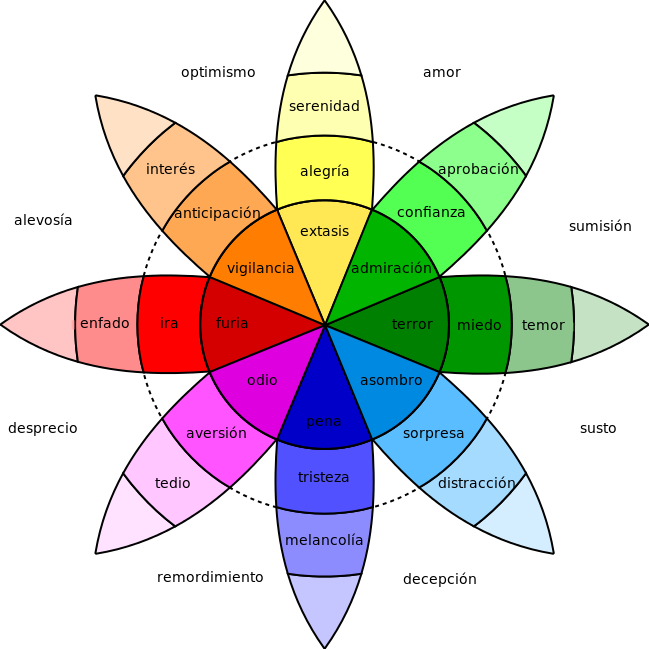
\includegraphics[width=0.7\textwidth]{plutchik-wheel.png}
\resizebox{0.75\textwidth}{!}{%
\begin{tikzpicture}[x=1.375cm,y=1.375cm]
\foreach \r in {4,3}
  \draw [dashed] circle [radius=\r];

%  {green!50!black, green!75!brown, yellow!50!white, orange, red, magenta, blue, blue!50!cyan}

\foreach \c [count=\i from 0] in  
  {gray!85!green, gray!85!brown, gray!85!yellow, gray!85!orange, gray!85!red, gray!85!magenta, gray!85!blue, gray!85!cyan}{
  \foreach \s [count=\j from 0] in {25,50,75,100}{
    \begin{scope}[rotate=\i*45]
      \clip (0,0) -- (22.5:2)
        arc (90:0:3 and 2*sin 22.5)
        arc (360:270:3 and 2*sin 22.5) -- cycle;
      \fill [fill=\c!\s!white] circle [radius=5-\j];
      \draw circle [radius=5-\j];
     \end{scope}
}}

\foreach \i in {0,...,7}
  \draw [rotate=\i*45] (0,0) -- (22.5:2)  
    arc (90:0:3 and 2*sin 22.5)
    arc (360:270:3 and 2*sin 22.5);

\foreach \emotionlist [count=\i] in
  {{terror,miedo,temor},
   {admiración,confianza,aprobación},
   {éxtasis,alegría,serenidad},
   {vigilancia,anticipación,interés},
   {furia,ira,enfado},
   {odio,aversión,tedio},
   {pena,tristeza,melancolía},
   {asombro,sorpresa,distracción}}
  \foreach \emotion [count=\j] in \emotionlist
    \node [anchor=base, font=\footnotesize, emotion label \i-\j/.try] at (\i*45-45:\j+.5) {\emotion};

\foreach \emotion [count=\i] in
{sumisión, amor, optimismo, alevosía,desprecio,remordimiento,decepción,susto}
  \node [anchor=base, font=\footnotesize]
    at (\i*45-22.5:4.75) {\emotion};

\end{tikzpicture}
}

	\caption[Rueda de las Emociones de Plutchik.]
	{\small Rueda de las Emociones de Plutchik. Cada rama representa una de las 8 emociones primarias y sus 3 niveles de intensidad.}
	\label{img:plutchik}
\end{figure}


\todojocelyn{no es posible integrar las secciones 2.4.2.1 y 2.4.2.2? dado que sigues hablando del trabajo de Dood ..}

\subsubsection{Relevancia histórica}
%% =====================================================================
% - Sobre concepto de relevancia historica
% - mezlcla y relevancia generalizada
% - algoritmo y graph
La relevancia histórica es un indicador que representa el olvido o pérdida de interés sobre un episodio en la memoria. Está directamente relacionado a la edad de un episodio, a menor antigüedad, mayor es su importancia, lo que se traduce en una mayor probabilidad de recordar ese episodio.

La implementación de relevancia histórica es estudiada por Dood et al., donde presenta una estrategia para su implementación y su interacción con la memoria emocional~\cite{Dodd2005}. Propone el uso de un indicador de relevancia generalizado, obtenido al combinar la intensidad de los dos indicadores. Además, propone un modelamiento matemático para representar el decaimiento de la relevancia histórica en el tiempo.

%\todounsure{Es necesario poner ecuaciones y curvas de decaimiento??}


\chapter{Diseño}\label{chapter:diseno}


En este capítulo se revisa el diseño del sistema LTM implementado en el proyecto. En primer lugar, se presentan todos los requerimientos para el diseño del sistema. A partir de éstos se elabora un conjunto de validaciones y pruebas que permitirán guiar el diseño, implementación y posterior evaluación del proyecto. Finalmente, y a partir de lo anterior, se diseña la arquitectura del sistema: se revisa el diseño de un episodio, el modelo de datos, el diseño del servidor, y el conjunto de complementos a implementar para la validación.
\unsure[inline]{Es correcto hablar de plugins?.. o debo usar ``complementos''?}


\todo[inline]{Modificar ocurrencias de campos What, When, Where por versiones \texttt{What, When, Where}} 

\section{Requerimientos}

A continuación se presentan los requisitos de diseño sobre los que se construye el proyecto. Primero se da una descripción breve sobre el origen y razón de los requisitos. Luego, se presenta un listado formal de todos los requerimientos, escritos de una forma clara y verificable.
 
\subsection{Definición de los requisitos (Requisitos de Usuario)}

\unsure[inline]{Está bien hablar sobre ``requisitos de usuario''??.. en realidad casi todos fueron inventados por mi durante la propuesta!! Yo soy mi propio cliente O.O ... }

\unsure[inline]{Qué tan formal debo ser con la especificación de req. usuario y req. software?? Si soy ultra formal (estilo curso Ing.Soft II) tendría que poner un documento de requisitos en los anexos.. mucha pega sin sentido?. Sólo quiero graduarme :'( }
%\subsubsection{Requisitos de capacidad}
%\subsubsection{Requisitos de calidad}
%\subsubsection{Requisitos de restricción}

El primer conjunto de requisitos se obtiene a partir de los objetivos del proyecto y sus alcances:
\begin{itemize}
\item Diseño de LTM (episódica y semántica) para robots de servicio domésticos.
\item Implementación integrada en Bender, compatible con su sistema.
\item Dar demostración de funcionalidades introducidas.
\item Énfasis en diseño de sistema genérico y compatible con más robots.
\item Memoria emocional debe ser soportada por el diseño, a pesar de no ser implementada.
\end{itemize}

El siguiente conjunto de requisitos corresponde a los 11 requerimientos para una memoria EpLTM planteados por Stachowicz\cite{Stachowicz2012} y presentados en la Sección \ref{sec:mem_robotica}. 

El sistema de relevancia episódica es importante para habilitar búsquedas de episodios según su importancia. En primer lugar, el sistema debe soportar el concepto de relevancia histórica de episodios, similarmente a lo estudiado por XXX \cite{} y presentado en la sección \ref{}. En cuanto a la relevancia emocional, el sistema debe permitir indexar episodios mediante este concepto. Además, se debe considerar que existen diversos sistemas de manejo de emociones, y el diseño no debe ser restrictivo respecto a ello. Finalmente, los episodios deben manejar un indicador de relevancia, que encapsule todos los demás indicadores en solo uno.
\todo[inline]{Al parecer, en el marco teórico no se habla sobre la relevancia histórica ni las metodologías para unir las relevancias.}
\todo[inline]{El indicador conjunto de relevancias aún no ha sido implementado}

\subsubsection{Alcances del proyecto}

\unsure[inline]{Es necesario hablar sobre cosas que NO SON REQUISITOS??}

Para acotar el diseño, implementación y validaciones, a continuación se presenta un listado requerimientos que no pertenecen al proyecto actual, sino que son considerados como trabajo futuro.

\begin{itemize}
\item Mecanismos para olvido o represión (en caso de contenido emocional traumático).
\item Problemas éticos sobre almacenar datos de usuarios.
\item Inferencia de información a partir de episodios almacenados.
\item Inferencia de episodios según sucesos previos y posteriores, como lo propuesto por Kelley \cite{Kelley2014} y estudiado en la Sección \ref{}.
\item Indicador de relevancia por novedad del episodio, basado en similitud con episodios ya existentes. No es de interés, pues se puede abstraer al módulo emocional.
\item Modificar conversaciones que mantiene el robot con humanos, según los datos episódicos almacenados (e.g., si se está hablando sobre una entidad nueva o ya conocida).
\item Eliminación automática de datos para liberar recursos de memoria secundaria.
\end{itemize}
\todo[inline]{En un principio se gastó tiempo con knowrob y prolog... que hago respecto a esto?? lo agrego al informe??... quito la inferencia de los objetivos secundarios??}

\todo[inline]{Reescribir requerimientos de diseño}

\todo[inline]{Agregar requerimientos basados en las pruebas que sobran}

\subsection{Requerimientos de software}

A continuación se presenta un listado (semiformal) de requisitos de software, generados a partir de los requisitos de usuario revisados en la sección anterior. Cada requisito de fue reformulado desde su versión difusa, a una descripción más precisa y verificable del requerimiento original. 
\unsure[inline]{Debo dar excusa sobre la informalidad del formato de presentación de requisitos?? Dan un poco de pena respecto a los visto en ING. Soft II, por ejemplo: link a requisito de usuario.. separación por tipo de requisito.. metadatos del requisito... matriz de trazabilidad... etc}

\paragraph{RS01}
El sistema debe ser agnóstico respecto a la plataforma objetivo. No se puede asumir que estructuras de datos semánticas serán almacenadas para cada episodio. Debe permitir que usuarios definan las estructuras de datos semánticas a almacenar.

\paragraph{RS02}
El servidor debe ser implantado en el robot Bender. Debe ser agregado al proceso de instalación y su documentación.Debe ser configurado para ser ejecutado simultáneamente a los otros módulos.

\paragraph{RS03}
Se deben implementar instancias de cada componente genérico, enfocadas en el robot Bender.
\begin{itemize}
	\item Implementación de la interfaz para adquisición de episodios basados en librería SMACH.
	\item Implementación de memoria semántica adecuada al robot: Información sobre personas y objetos.
	\item El software dedicado al robot debe ser implementado en paquetes de ROS distintos del utilizado para el servidor LTM.
\end{itemize}

\paragraph{RS04}
El servidor debe ser compatible con ROS, mediante una API ROS para acceder a todas sus funcionalidades.

\paragraph{RS05}
El servidor debe proveer servicios para las operaciones CRUD sobre los episodios manejados.

\paragraph{RS06}
Los episodios almacenados deben estar conectados bidireccionalmente con los datos semánticos relacionados.

\paragraph{RS07}
(R1) Episodios deben contener campo What, para almacenar memoria semántica. Ya que la memoria semántica es definida por el usuario, éste campo debe poder almacenar cualquier tipo de información.

\paragraph{RS08}
(R1) Episodios deben contener campo When, para almacenar tiempos de inicio y finalización del episodio. Debe poder manejar intervalos de tiempo desde segundos a años.

\paragraph{RS09}
(R1) Episodios deben contener campo Where, para almacenar información sobre la ubicación del robot durante su ocurrencia.

\paragraph{RS10}
(R2) Episodios deben ser indexados al menos por los campos What, When y Where.
\todo[inline]{Cómo valido esto?}

\paragraph{RS11}
(R2) El servidor debe permitir realizar búsquedas de episodios con condiciones sobre la información almacenada para What, When, Where. Las condiciones de búsqueda deben permitir comparaciones {igualdad, mayor que, pertenencia} entre tipos de dato básicos {strings, números, bool}, asociados a los campos del episodio.

\paragraph{RS12}
(R3) Los episodios pueden crear entidades semánticas o actualizar las ya existentes.

\paragraph{RS13}
(R4)  Cada episodio ingresado a la memoria es único, a pesar de que existan similitudes con otros episodios.

\paragraph{RS14}
(R5) A partir de un episodio se puede acceder a episodios padre e hijos.

\paragraph{RS15}
(R6)  Lecturas de episodios deben mostrar la memoria semántica como se conocía en ese instante. Es decir, resultado de la consulta debe mostrar los campos asociados a entidades, como si nunca más hubieran cambiado.)

\paragraph{RS16}
(R7) Episodios pueden estar compuestos de sub-episodios.

\paragraph{RS17}
(R8) Pueden existir episodios simultáneos, y con distintos tiempos de inicio y fin.

\paragraph{RS18}
(R9) Se deben minimizar las dependencias de módulos de software externos para el funcionamiento del servidor. Particularmente:
El sistema debe ser implementado en ROS y solamente utilizando las librerías estándar de Python y C++. La única excepción corresponde a la librería para el manejo de la base de datos a utilizar.
No deben existir dependencias extra para los módulos de memoria semántica definidos por el usuario, ni para la representación de la memoria semántica.

\paragraph{RS19}
(R9) En caso que ya exista información semántica almacenada, los usuarios deben poder modificar su representación.

\paragraph{RS20}
(R10) El servidor debe tolerar una alta tasa de generación de eventos, sin degradar el funcionamiento del robot. Específicamente:
\todo[inline]{Esos valores de recursos fueron escogidos al azar!.. deben ser modificados.}
\begin{itemize}
	\item El funcionamiento base del sistema, es decir, con el servidor en ejecución y sin consultas funcionando, no debe exceder el uso del 15\% del CPU y 15\% de RAM del la plataforma objetivo.
	\item Debe poder manejar al menos la generación de 10 eventos simultáneamente, sin exceder un aumento en el uso de recursos de un 10\%, relativo al costo de su funcionamiento base.
	\item En caso de que el robot tenga más del 90\% de sus recursos de CPU ocupados, el sistema debe entrar en modo de bajo consumo, y encolar los episodios para posterior almacenamiento.
\end{itemize}


\paragraph{RS21}
(R11) Costos de operaciones CRUD deben escalar bien, respecto a la cantidad de datos almacenados. Particularmente, el costo en tiempo de las operaciones debe estar acotado en $O(n\ log\ n)$ respecto a la cantidad de episodios almacenados.

\paragraph{RS22}
Episodios deben tener un indicador numérico de relevancia histórica, el que debe ser degradado automáticamente con el paso del tiempo.

\paragraph{RS23}
Episodios deben tener, al menos, la siguiente información sobre la emoción del robot asociada al episodio: nombre de la emoción principal asociada, e indicador numérico que identifique la intensidad de la emoción. La estructura de datos y formato utilizado no debe depender de algún software emocional externo.

\paragraph{RS24}
Episodios deben tener un indicador numérico de relevancia episódica generalizado, que una los subsistemas de relevancia en sólo uno. El indicador debe ser actualizado automáticamente cuando cualquiera de los subindicadores sea actualizado.

\paragraph{RS25}
El robot Bender no dispone de módulos para el cómputo de emociones. Se deben implementar al menos 3 sistemas de generación de emociones para el robot, los que deben ser utilizados para la demostración.

\paragraph{RS26}
Episodios deben estar indexados por los siguientes indicadores numéricos de relevancia, sumado a la descripción de la emoción. Se deben poder realizar búsquedas utilizando éstos índices.

\unsure[inline]{Requisito sobre que la implementación de la interfaz episódica implementada en SMACH debe ser lo menos instrusiva posible.}

\unsure[inline]{Requisito sobre que la implementación de la interfaz episódica implementada en SMACH no debe fallar / colgarse / arrojar excepciones por ningún motivo, para no sacrificar el funcionamiento del robot en caso de errores.}

\section{Validaciones}

A continuación se presenta un conjunto de validaciones para la implementación del sistema. Éstas son generadas directamente desde los requisitos planteados anteriormente, y además sirven como guía para el diseño e implementación del proyecto. Éstas se separan en 4 categorías: 1. Validaciones que se verifican directamente desde el diseño e implementación del sistema, 2. validaciones mediante la ejecución del sistema, 3. validaciones mediante consultas episodicas al servidor, y 4. validaciones mediante pruebas de estrés al servidor.

\todo[inline]{listado formal de validaciones basadas en requerimientos}

\subsection{Validaciones por diseño e implementación}
\paragraph{VA01 (RS01)}
% estado [OK]
Verificar que el que el proyecto no tiene ninguna dependencia en software propio del robot.

\paragraph{VA02 (RS01)}
% estado [OK]
Verificar que el servidor admite la definición de estructuras de datos genéricas para la información semántica.

\paragraph{VA03 (RS02)}
% estado [PENDING]
Verificar que el sistema LTM se encuentra documentado en la documentación del robot. La documentación debe incluir tutoriales de instalación y uso del sistema.

\paragraph{VA04 (RS03)}
% estado [PENDING]
Verificar que existan implementaciones de entidades semánticas para personas y objetos.

\paragraph{VA05 (RS03)}
% estado [OK]
Verificar que módulos de software implementados sean separados en al menos 2 paquetes de ROS. El primero debe contener el servidor LTM sin ninguna dependencia al robot. El resto debe contener los módulos extra implementados y deben depender del primero.

\paragraph{VA06 (RS07)}
% estado [OK]
Verificar que el campo What de un episodio pueda almacenar cualquier estructura de datos que ROS sea capaz de manejar.

\paragraph{VA07 (RS08)}
% estado [OK]
Verificar que episodios poseen campo When, para almacenar tiempo de inicio y finalización del episodio

\paragraph{VA08 (RS13)}
% estado [OK]
Verificar que cada nuevo episodio disponga de un ID único entre el resto de los episodios ya almacenados.

\paragraph{VA09 (RS18)}
% estado [OK]
Verificar que el paquete de ROS que implementa el servidor sólo tenga como dependencias: librerías estándar de C++ y Python, driver de la base de datos, paquetes estándar de ROS.


\paragraph{VA10 (RS23)}
% estado [OK]
Verificar que estructura de datos emocional sólo está compuesta por tipos de datos disponibles entre los del estándar en ROS. Verificar que el sistema LTM sólo dependa de la intensidad de la emoción y nombre asociado para la implementación de sus funcionalidades.


\subsection{Validaciones mediante ejecución}

\paragraph{VB01 (RS02)}
% estado:  [PENDING]
Verificar que el sistema LTM se instala correctamente en conjunto con la instalación del robot.

\paragraph{VB02 (RS02)}
% estado:  [PENDING]
Verificar que tras iniciar el software base del robot, se encuentre activo el servidor LTM y sus API ROS.

\paragraph{VB03 (RS03)}
% estado:  [OK]
Verificar que servidor almacena episodios generados a partir de la interfaz con SMACH. Se debe verificar que un set de máquinas de estado ejecutadas sea procesado correctamente.

\paragraph{VB04 (RS04)}
% estado:  [OK]
Verificar que el paquete ROS provee herramientas para lanzar el servidor.

\paragraph{VB05 (RS04)}
% estado:  [OK]
Verificar que el servidor provee API ROS para configurar sus parámetros.

\paragraph{VB06 (RS05)}
% estado:  [PENDING]
Verificar que el servidor activo provee API ROS para agregar, buscar, actualizar y borrar episodios. 

\paragraph{VB07 (RS25)}
% estado:  [PENDING]
Verificar que existan implementados al menos 3 módulos generadores de emociones para el robot Bender. Éstos deben utilizar sensores disponibles en el robot. Los módulos deben pertenecer a un paquete de ROS dedicado.


\subsection{Validaciones mediante consultas al servidor}

\paragraph{VC01 (RS03)}
% estado:  [TOO BROAD]
\todo{TO DO}
Consultas relacionadas a entidades de personas y objetos!

\paragraph{VC02 (RS06)}
% estado:  [PENDING]
Obtener un episodio desde el servidor. A partir de él, acceder a datos semánticos definidos. Verificar que se pueda obtener referencia al episodio a partir de los datos semánticos obtenidos.

\paragraph{VC03 (RS06)}
% estado:  [PENDING]
Obtener una entidad desde el servidor. A partir de ella, listar todos los episodios relacionados.

\paragraph{VC04 (RS08)}
% estado:  [OK]
Verificar que el servidor permita almacenar episodios con duraciones de segundos, horas, días y años.

\paragraph{VC05 (RS09)}
% estado:  [TOO BROAD]
\todo{TO DO}
Verificar que episodios contengan campo Where. Almacenar episodios utilizando distintas ubicaciones.

\paragraph{VC06 (RS11)}
% estado:  [PENDING]
\todo{TO DO}
Test R02: Search: Buscar episodios indexados por W-1.
Test R03: Search: Buscar episodios indexados por W-2.
Test R04: Search: Buscar episodios indexados por W-3.


\paragraph{VC07 (RS12)}
% estado:  [PENDING]
\todo{TO DO}
(R3 Flexibilidad)
Test R05: Preguntar por datos aprendidos posteriormente.
A: Interactúa con (a) y lo almacena.
B: Interactúa con (a) o (b) y aprende dato sobre (a).
C: Consulta sobre (a) muestra nuevo dato.
Test R06: Preguntar por datos modificados posteriormente.
A: Interactúa con (a) y lo almacena.
B: Interactúa con (a) o (b) y modifica dato sobre (a).
C: Consulta sobre (a) muestra dato modificado.


\paragraph{VC08 (RS14)}
% estado:  [OK]
Obtener un episodio desde el servidor. A partir de sus datos consultar por su episodio padre y episodios hijos.

\paragraph{VC09 (RS15)}
% estado:  [PENDING]
\todo{TO DO}
(R6: Perspectiva)
Test R10: Eventos recordados deben mantener perspectiva de la experiencia original.
Episodio A: Habla con (a). Almacena que es estudiante de colegio.
Episodio B: Habla con (a). Almacena que es estudiante de U.
Recordar A: debe decir que (a) era estudiante de colegio.
Recordar B: debe decir que (b) era estudiante universitario. 

\paragraph{VC10 (RS16)}
% estado:  [OK]
\todo{TO DO}
Test R11: Evento A con sub evento B (temporalmente)



\paragraph{VC11 (RS17)}
% estado:  [OK]
Generar dos eventos transpuestos en tiempo (campo \texttt{When}). Verificar que al obtener ambos eventos, sus datos sean correctos y no se haya mezclado la información semántica asociada.


\paragraph{VC12 (RS19)}
% estado:  [PENDING]
Crear entidad semántica para el test con estructura A. Crear e ingresar M episodios que ocupen la estructura A. Modificar entidad y dejar en estructura B. Ingresar N episodios que utilicen estructura B. Realizar búsquedas de episodios con estructura A y de episodios con estructura B.


\paragraph{VC13 (RS22)}
% estado:  [PENDING]
Generar episodios con antigüedades en el rango de 1 segundo hasta 5 años, espaciados por intervalos de horas (para los 24 primeros) y días, para los (365) siguientes y semanas para el resto. Forzar actualización de relevancias, leer todos los episodios y graficar su relevancia histórica, para verificar que es decreciente.

\paragraph{VC14 (RS23)}
% estado:  [PENDING]
Consultar algún episodio de la base de datos. Verificar que dispone de campos de relevancia emocional: Indicador numérico para la intensidad de la emoción, y descripción de la emoción.

\paragraph{VC15 (RS24)}
% estado:  [PENDING]
Consultar algún episodio de la base de datos. Verificar que dispone de un indicador numérico con la relevancia generalizada.
\begin{itemize}
\item Verificar que al disminuir la relevancia histórica del episodio, la relevancia generalizada también disminuya.
\item Manteniendo las otras relevancias fijas. Verificar que episodios con mayor/menor relevancia emocional muestran una mayor/menor relevancia generalizada.
\item Manteniendo las otras relevancias fijas. Verificar que episodios con mayor/menor relevancia histórica muestran una mayor/menor relevancia generalizada.
\end{itemize}

\paragraph{VC16 (RS25)}
% estado:  [PENDING]
Generar episodios en donde se ocupe cada uno de los módulos generadores de emociones implementados para el robot Bender.

\paragraph{VC17 (RS26)}
% estado:  [PENDING]
Generar episodios con distintos índices de relevancia histórica, emocional y generalizada. Verificar que se puedan realizar búsquedas de episodios mediante cada uno de los indicadores de relevancia, sumado a la descripción de la emoción.

\subsection{Validaciones de eficiencia}

\todo[inline]{Reescribir validaciones una vez estas se hayan ejecutado!.}

\todo[inline]{Revisar pruebas de eficiencia de Stachowicz \cite{Stachowicz2012}, y Vijayakumar \cite{Vijayakumar2014}. Agregar referencia a sus evaluaciones.}

\todo[inline]{Escribir en algún lado a que me refiero con estado/funcionamiento base.}

Las siguientes validaciones tienen por objetivo medir la eficiencia del sistema LTM una vez implementado, y se construyen a partir del requisito de software (RS20). Cada una busca medir el uso de algún recurso del sistema, mientras el servidor se encuentra en funcionamiento y en espera. 

Se deben realizar las siguientes mediciones:
\begin{enumerate}
\item Uso de CPU y RAM cuando el servidor está en estado base.
\item Uso de CPU, RAM y ancho de banda de disco, para consultas de búsqueda episódica (simples) a tasas de \{0.5, 1, 2, 3, 4, 5, 6, 7, 8, 9, 10\}[Hz].
\item Uso de CPU, RAM y ancho de banda de disco, para consultas de búsqueda episódica (complejas) a tasas de \{0.5, 1, 2, 3, 4, 5, 6, 7, 8, 9, 10\}[Hz].
\item Uso de CPU, RAM y ancho de banda de disco, para servicio de ingreso de episodios (sin información semántica), a tasas de \{0.5, 1, 2, 3, 4, 5, 6, 7, 8, 9, 10\}[Hz].
\item Uso de CPU, RAM y ancho de banda de disco, para servicio de ingreso de episodios (con información semántica), a tasas de \{0.5, 1, 2, 3, 4, 5, 6, 7, 8, 9, 10\}[Hz].
\end{enumerate}
\todo[inline]{hablar sobre simple/complejo es muy subjetivo.}

\paragraph{VD01 (RS20)}
En primer lugar, se debe validar que en estado base, el uso de CPU y RAM no exceda al 15\% del total disponible para el robot Bender.

\paragraph{VD02 (RS20)}
Se debe verificar que las operaciones de búsqueda no sobrepasen el uso de recursos en un 10\%, respecto al costo del funcionamiento base. Es decir, se admite hasta un 25\% del uso del total de recursos disponibles para el robot.
\todo[inline]{Actualizar requerimiento para considerar ancho de banda del disco y agregar validación asociada.}

\paragraph{VD03 (RS20)}
Verificar que si al menos un 90\% de los recursos de CPU del robot se encuentran ocupados, el servidor LTM entra en modo de bajo consumo. En éste modo, el servidor no puede ocupar más del 5\% de recursos extra a los de su estado base, y todas las consultas deben ser postergadas.
\todo[inline]{Corregir esto: no tiene sentido postergar consultas de búsqueda.. sólo las de inserción!... (acumular episodios en RAM mientras) por último quitar este requerimiento!.}


\subsection{Validaciones de escalabilidad}

Las siguientes conjuntos de validaciones se construyen a partir del requisito de software (RS21). Tienen por objetivo medir el costo de tiempo de las operaciones de inserción, búsqueda y borrado de episodios, en función de la cantidad de episodios almacenados en la base de datos. En cada una se busca validar que la complejidad temporal de las operaciones se comporte de la forma $\mathcal{O}(n\log{}n)$.

\todo[inline]{Revisar pruebas de escalabilidad de Stachowicz \cite{Stachowicz2012}, y Vijayakumar \cite{Vijayakumar2014}. Agregar referencia a sus evaluaciones.}

\todo[inline]{Verificar que complejidad escogida tiene sentido!.}

\begin{itemize}
\item {\bf VE01 (RS21)}: Tiempo de búsqueda vs. cantidad de episodios, según el campo \textit{What}
\item {\bf VE02 (RS21)}: Tiempo de búsqueda vs. cantidad de episodios, según el campo \textit{Where}
\item {\bf VE03 (RS21)}: Tiempo de búsqueda vs. cantidad de episodios, según el campo \textit{When}
\item {\bf VE04 (RS21)}: Tiempo de búsqueda vs. cantidad de episodios, según el campo \textit{What, When, Where}
\item {\bf VE05 (RS21)}: Tiempo de inserción vs. cantidad de episodios.
\item {\bf VE06 (RS21)}: Tiempo de borrado vs. cantidad de episodios.
\end{itemize}
\unsure[inline]{Quizás las validaciones de búsqueda tienen más sentido al buscar por el tipo del campo (número, string, bool)}
\unsure[inline]{Quizás las validaciones de inserción deban ser separadas en casos con pocos-muchos streams-entidades... y caso en vacío... Finalmente todo dependerá de la calidad de la implementación del usuario.. pero tiene sentido validar los plugins que si se implementarán en el robot.}
\unsure[inline]{Creo que el tiempo de borrado no tiene sentido!, actualización quizás... pero no es una operación común... las operaciones comunes deben ser sólo inserción y búsqueda}

\unsure[inline]{No estoy seguro si tiene sentido agregar validaciones de escalabilidad en el uso de recursos del sistema: CPU, RAM, DISCO}
%El segundo conjunto estudia el uso de recursos del sistema: CPU, disco y RAM.
%\paragraph{VE07 (RS21)}: disk usage vs. \# episodes
%\paragraph{VE08 (RS21)}: RAM usage vs. \# episodes
%\paragraph{VE09 (RS21)}: CPU usage vs. \# episodes



 
\section{Arquitectura del sistema}
 
 En esta sección se describe la el diseño de la arquitectura del sistema de software implementado, según los requerimientos estudiados anteriormente. En primer lugar se revisa el diseño de los episodios, su estructura de datos y limitantes. Luego se estudia el diseño del modelo de datos para la memoria episódica y su relación con los componentes semánticos. En tercer lugar se presenta el diseño del servidor LTM y sus limitantes. Finalmente, se definen la interfaz episódica y los componentes a implementar para la validación y demostración del proyecto.
 
 
\subsection{Diseño de episodios}
% - Diseño de episodios según requisitos
 .
 
\subsubsection{Árboles de episodios}
%    - Contexto
% - episodios son únicos.. por mucho que un hijo se parezca a otro.. son distintos
%    - manejo de datos episodicos en hijos
%    - construcción de padres a partir de los hijos
 .
 
\subsubsection{Contexto espacio-temporal}
%    - manejo de ubicación
%    - manejo de when
 .

\subsubsection{Manejo de relevancia emocional}
%    - diseño de sistema emocional
 .

\subsubsection{Manejo de relevancia histórica}
%    - manejo de datos historicos
 .

\subsubsection{Datos para introspección}
%    - manejo de otros datos
%    - otros datos para debugging e introspección
 .

\subsubsection{Memoria semántica}
%    - streams vs entidades
 .

\subsubsection{Limitantes}
%    - Limitantes:
%       - ubicación y frames
%       - padres mantienen con mismo frame y mapa de hijos
%       - contexto: introducción manual? TO DO
 .


\subsection{Diseño del modelo de datos}
% - Diseño de Base de Datos:
 .

\subsubsection{Consideraciones}
%    - manejo de colecciones y mensajes
%       - límite de tamaño de datos
%    - separación de colecciones para optimizar manejo de datos y memoria.
%       - optimizar queries comunes
%       - poder bloquear/eliminar colecciones muy pesadas
%    - otras funcionalidades de interés: bkp, migrate a otro robot, ...
%    - modificar msg de colección MD5 y poder seguir ocupando la base de datos.
%    - funcionalidades y limitantes de Mongo y de mongo_ros
%    - sistema de queries disponibles finalmente.
 .

\subsubsection{Colección de episodios}
%    - episodio
%    - mensaje ROS
 .

\subsubsection{Colecciones de streams}
%    - streams
%       - funcionalidad de streams. Separación de entidades.
%       - degradación
 .

\subsubsection{Colecciones de entidades}
%    - entidades
%       - cómo cumplir reglas sobre flexibilidad y perspectiva. Audit trail.

 .

\subsection{Diseño del servidor LTM}
%    - TODO: manejo de contexto
 .

\subsubsection{Manejo de episodios}
% - Diseño del servidor LTM según requisitos
%    - uso de MongoDB
%    - Minimizar dependencias
%    - API ROS: servicios, parámetros, nodos
 .

\subsubsection{Sistema de plugins}
%    - Sistema de plugins para agregar cosas específicas a cada robot
%        - requerimientos para cada plugin
%        - uso esperado de pluginlib
%        - flujo de trabajo de cada plugin
 .

\subsubsection{Alcances y trabajo futuro}
%    - Alcances y trabajo futuro
%        - reservar ids mientras nodo esté activo.
%        - posibles funcionalidades de interés: 
%           - visualizador
%           - 
 .

\subsection{Diseño de plugins e interfaces para demostración}
% - Plugins a implementar a modo de ejemplo, adecuados al robot bender.
 .

\subsubsection{Generación de episodios mediante SMACH}
%    - Smach: consideraciones
 .

\subsubsection{Plugin para obtener localización del robot}
 .

\subsubsection{Plugin para obtener emociones del robot}
 .

\subsubsection{Plugin para streams: Imágenes}
%    - Streams: dar ejemplos: img, sonido, pcl..
 .

\subsubsection{Plugins para entidades}
%    - Entidades: People, Objects, Robot, Location
 .


\chapter{Implementación}\label{chapter:implementacion}

\todowrite{Descripción del capítulo}

\todowrite{Agregar referencia al github de cada package y tutoriales respectivos.}

\section{Test suites}
% - Episodios JSON: comprensión de la estructura a utilizar
% - Episodios Smach: cubrir todos los casos de borde
% - Robot simulado: emociones y localización fakes
% - Streams Fake: videos
% - Entidades Fake: Generador de campos para mensajes

\section{Servidor LTM}
% - Mensajes
% - Genérico
% - Base de datos
% - Servicios
% - Plugins

\section{Módulos particulares a la simulación}
% - Interfaz Smach
%    - consideraciones iniciales
%    - Implementación sin impacto en librería y que minimiza trabajo del equipo
%    - consideraciones: no morir ante nada!
% - Interfaz Robot: Emociones y Posición
% - Plugin Streams
% - Entidades
% - Tutoriales

\section{Módulos particulares al robot}
% - Funcionalidades implementadas en el robot: 
%    - emociones simples.
%    - módulos disponibles (con el robot a medias)
% - Integración de ltm al sistema de UChile ROS Framework
%    - instalación y convivencia con el software
%    - visualización de datos episódicos.
% - Interfaz Smach
% - Interfaz Robot: Emociones y Posición
% - Streams
% - Entidades

\chapter{Resultados y Análisis}\label{chapter:results}

\todo[inline]{RESULTADOS: Escribir al cuando existan}

\section{Ambiente de simulación}
% - 
% - 
% - 

\section{Validaciones}
% - 
% - 
% - 

\section{Simulación completa}
% - 
% - 
% - 

\section{Simulación y robot}
% - 
% - 
% - 
\begin{conclusion}

% OVERVIEW
En este trabajo se diseñó e implementó una memoria episódica de largo plazo para robots domésticos basados en ROS. El trabajo estuvo enfocado en el diseño de un sistema LTM adecuado a Bender, pero capaz de ser integrado en otras plataformas robóticas que utilizan ROS.

% RELEVANCIA
En primer lugar, se estudió la relevancia de una memoria a largo para un robot doméstico. Este concepto es esencial para mejorar el desempeño de las tareas que debe realizar el robot. Más aún, esta capacidad tiene un alto impacto en la interacción humano-robot, permitiendo comportamientos interesantes y evitando la pérdida de interés del operador. Es decir, la memoria LTM es esencial para un robot doméstico.

% INVESTIGACION
Según se investigó, hay pocos trabajos enfocados en este tema y aún no existe un consenso respecto a la implementación de un sistema LTM. Sin embargo, algunos trabajos siguen una serie de requerimientos básicos para un sistema de este tipo. El diseño estuvo fuertemente influenciado por los requerimientos episódicos propuestos por Stachowicz, que rigen el comportamiento del sistema y las cualidades esperadas del mismo.

% DISEÑO
De los objetivos del trabajo se derivaron requisitos de sistema y validaciones con las que guiar el diseño e implementación. El sistema LTM diseñado permite recolectar episodios a través de máquinas de estado, las que son utilizadas comúnmente para la implementación de comportamientos en robots domésticos. Cada episodio está asociado a información semántica, en forma de streams y entidades, cuya representación debe ser definida por el usuario y sus datos recopilados mediante un sistema de plugins implementados por él. De esta forma, el sistema LTM puede ser integrado en Bender, pero también en otros robots basados en ROS. El costo de la generalidad que provee el sistema es que se dejan muchas decisiones de implementación al usuario, lo que puede ser problemático cuando hay errores en un plugin, o para asegurar un desempeño similar en cada caso de uso.

% IMPLEMENTACIÓN
El sistema LTM provee una API ROS para su ejecución, configuración y recolección de episodios. Utiliza la base de datos MongoDB para el almacenamiento de episodios. Utilizando el lenguaje de consulta de MongoDB, el sistema permite realizar búsquedas de episodios mediante cualquier combinación de condiciones lógicas.


% RESULTADOS
Para el caso de uso de Bender, los experimentos muestran que el costo temporal de las consultas episódicas escala linealmente respecto a la cantidad de episodios almacenados, siendo capaz de responder un conjunto de consultas de interés en menos de 0.25[s] a los 10 años de uso. En términos de eficiencia, el sistema LTM es capaz de mantener una tasa de 600 consultas por minuto, llegando a utilizar el 20\% de CPU y de 200 consultas por minuto, utilizando el 5\%. En ambos experimentos, el sistema LTM cumple los requerimientos para el caso de uso estudiado, sin embargo, queda claro que la consulta a utilizar debe ser elegida adecuadamente, pues la duración de esta puede comprometer la fluidez de una interacción humano-robot y además, puede saturar el núcleo de CPU asignado.

% REQs FUNCIONALES
El sistema LTM cumple con todos los requisitos funcionales establecidos, a excepción de 2 puntos. Primero, aún no se implementa la capacidad de migrar la base de datos a una nueva estructura semántica. Segundo, se requiere un algoritmo para la actualización automática de la relevancia histórica y generalizada, esto se revisa en el capítulo de diseño, pero no ha sido implementado. Ambos puntos permitirían concluir la implementación y se consideran parte del trabajo futuro.

% INTEGRACIÓN CON BENDER
Respecto a la integración del sistema LTM en el robot Bender, esta es parcial. Se integraron correctamente los plugins para recolección de imágenes y de la localización del robot, junto a la interfaz para recopilar episodios a partir de máquinas de estado en SMACH. Se realizaron las modificaciones requeridas en URF para instalar y ejecutar el sistema junto al robot. Sin embargo, no se pudo acceder al robot para completar la integración, dejando de lado el plugin para la recopilación de entidades y del estado emocional.
\todojavier{actualizar???}

% FINALMENTE
Finalmente, se considera este trabajo como una oportunidad de promover la inclusión de desafíos basados en sistemas LTM en la liga RoboCup@Home. Para ello, a partir de las investigaciones y diseño realizado, se ha elaborado un estudio~\cite{ltm_in_robocup} motivando el uso de LTM y una metodología para su inclusión en la competencia. Así, se espera que el desarrollo de LTM y capacidades asociadas deje de ser postergado y pase a ser una de las prioridades para los equipos participantes.


\section*{Trabajo Futuro}

El trabajo realizado provee un servidor LTM genérico para robots domésticos. El sistema cumple con los requisitos básicos que una memoria episódica debiera cumplir, sin embargo, hay muchos aspectos pendientes o no cubiertos por este trabajo.

En primer lugar, el trabajo futuro más importante es la implementación de los aspectos dejados como pendientes. Es decir, la migración de la base de datos, el algoritmo para la actualización automática de relevancias, el plugin para entidades y el sistema emocional de Bender.

Ya que la selección de una consulta episódica puede tener un alto impacto en el desempeño del sistema, se considera prioritario realizar un estudio sobre el costo de cada operación lógica que provee MongoDB y sus interacciones. Esto, con el fin de optimizar las consultas y asegurar una medida de desempeño del sistema LTM. Por otro lado, los experimentos de desempeño pueden ser complementados con casos de uso de streams y entidades, y mediciones sobre la tasa de lectura y escritura de memoria secundaria.

La inferencia de información a partir de los recuerdos también es un aspecto deseable. Esto fue considerado en primera instancia para el desarrollo del trabajo, pero tras algunas pruebas preliminares no se pudo satisfacer este objetivo secundario, debiendo acotar el alcance del trabajo. La propuesta consideraba el uso del framework KnowRob~\cite{Winkler2014,Tenorth2013,Tenorth2009}, que implementa memoria semántica y permite inferir información a partir de los datos almacenados.



\end{conclusion}
\begin{glosario}\label{chapter:glosario}

\todoimprove{Revisar \url{https://es.sharelatex.com/learn/Glossaries}}

\todounsure{Agregar cosas en cursiva?, cosas en inglés y siglas.}

\todowrite{Buscar doc por ocurrencias de estos puntos y asegurar que son descritos en primera instancia.}

\begin{itemize}
\item LTM: Long Term Memory.
\item API: Application Programming Interface
\item ROS: Robot Operating System
\item plugin
\item stream
\item driver
\item launchfile
\item tópico
\item buffer
\end{itemize}

\end{glosario}	


\bibliographystyle{IEEEtran}
\bibliography{IEEEabrv,bibliography}
%\bibliographystyle{plain}
%\bibliography{bibliografia}

\end{document}
